\documentclass[12pt]{scrartcl}

\usepackage[english, francais]{babel}
\usepackage[T1]{fontenc}
\usepackage[utf8]{inputenc}
\usepackage{lmodern}
\usepackage{graphicx, caption}
\usepackage{amssymb}
\usepackage{graphics, caption}
\usepackage{mathtools, bm}
\usepackage{hyperref}
\usepackage{xlop}
\usepackage{changepage}
\usepackage{tabvar}
\usepackage{afterpage}
\usepackage{amsmath}
\usepackage{bbold}
\usepackage{slashbox}
\usepackage{apacite}
\usepackage{lipsum}
\usepackage{listings}
\usepackage{color}
\usepackage{url}

\makeatletter\@addtoreset{section}{part}\makeatother
\renewcommand{\thesection}{\arabic{section}}

\newcommand{\dd}{\mathrm{d}}
\DeclareMathOperator{\e}{e}

% Default fixed font does not support bold face
\DeclareFixedFont{\ttb}{T1}{txtt}{bx}{n}{12} % for bold
\DeclareFixedFont{\fnb}{T1}{txtt}{bx}{n}{10} % for bold

% Custom colors
\usepackage{color}
\definecolor{deepblue}{rgb}{0,0,0.5}
\definecolor{deepred}{rgb}{0.6,0,0}
\definecolor{deepgreen}{rgb}{0,0.5,0}

% Python style for highlighting
\lstset{
language=Python,
basicstyle=\ttfamily,
otherkeywords={self}, % Add keywords here
keywordstyle=\ttb\color{deepblue},
stringstyle=\color{deepgreen},
commentstyle=\color{deepred},
frame=tb, % Any extra options here
showstringspaces=false, % 
tabsize=2
}

\newcommand\blfootnote[1]{%
\begingroup
\renewcommand\thefootnote{}\footnote{#1}%
\addtocounter{footnote}{-1}%
\endgroup
}

\renewcommand{\lstlistingname}{Programme}% Listing -> Algorithm
\renewcommand{\lstlistlistingname}{List of \lstlistingname s}% List of Listings -> List of Algorithms

\renewcommand{\labelenumii}{\theenumii}
\renewcommand{\theenumii}{\theenumi.\arabic{enumii}.}

\usepackage{empheq}

\title{Modélisation mathématique et informatique de neurones : création d'une bibliothèque Python/Tensorflow pour la simulation de réseaux de spiking-neurons et applications }
\subtitle{Dans une idée de rapprochement entre la modélisation du système nerveux et l'intelligence artificielle}
\author{Granier Arno \\ encadré par C.Shlick et B.Ainseba}

\begin{document}

\maketitle

\tableofcontents

\pagebreak


\part{Introduction}
\blfootnote{nldr : dans ce travail on va souvent assimiler, par facilité de rédaction, l'homme à son système nerveux, ou à son système cognitif. On essaiera d'employer le terme "système nerveux" plutôt que "cerveau" ou "encéphale", pour rester général et conserver l'importance du système nerveux périphérique. On utilisera souvent également les mots cognition et esprit avec le même sens.}

Les sciences cognitives sont un hybride de plusieurs disciplines inter-résonnantes, chacune comportant ses propres préoccupations et engagements, et appartenant à des champs de recherche très divers, allant de la philosophie aux mathématiques, en passant par la psychologie et les sciences naturelles. Dans le travail qui va suivre, bien que le discours va presque toujours appartenir aux sciences formelles et naturelles, l'intention est bien celle qui fait les sciences cognitives, c'est-à-dire d'étudier, d'expliquer la cognition, l'esprit humain. Plus précisément, l'intention ici est de s'intéresser à une idée d'explication de l'Homme et de son esprit en des termes des sciences formelles et naturelles. Nous allons voir dans cette introduction comment cela est envisageable, mais d'abord, j'aimerais dire que je ne pense pas qu'il soit souhaitable (sans parler de la faisabilité) d'essayer de réduire l'homme à son étude du point de vue des sciences formelles et naturelles, et je pense qu'au contraire une étude de multiples points de vue est ce qui nous rapprochera le plus d'une compréhension de l'homme, de son esprit et de sa culture.\\

Le développement de disciplines comme la psychophysiologie ou plus généralement les neurosciences nous permet d'envisager une naturalisation de la cognition humaine, de l'esprit humain (ou du moins d'une partie de cette cognition, de cet esprit). Dire qu'on peut naturaliser la cognition, c'est dire que la cognition humaine serait explicable en des termes des sciences naturelles, notamment à travers la biologie et la physique du système nerveux humain. On s'inscrit alors dans un courant naturaliste, voire physicaliste. Cela permettrait d'étudier l'esprit, la cognition de la même manière que n'importe quel autre objet des sciences naturelles (ou physiques), et on aurait de plus une explication possible des états mentaux humains par certaines propriétés de la matière. Mais, et en accord avec une théorie fonctionnaliste, on ne va pas définir les états mentaux par ces propriétés de la matière, mais plutôt par la fonction de ces états mentaux au sein du mental ou au sein de l'organisme, la matière n'étant que la base permettant la réalisation de cette fonction. Avec cette approche physicaliste-fonctionnaliste, il est donc théoriquement envisageable de reproduire le système cognitif, l'esprit humain dans une machine, pourvu que l'on reproduise toutes les propriétés physiques du système nerveux humain, le physicalisme nous permettant d'attribuer entièrement l'esprit humain aux propriétés physiques du système nerveux humain, et le fonctionnalisme nous permettant de nous affranchir d'une incarnation forcément dans le système nerveux pour nous étendre à une incarnation possible dans tout système \textit{fonctionnant comme} le système nerveux. \\

Mais qu'est-ce que ça veut dire \textit{fonctionner comme} le système nerveux ? Pour répondre à cette question, il nous faut nous tourner vers les sciences naturelles : neurosciences, biologie, physique, etc., qui étudient les propriétés biologiques, chimiques et physiques du cerveau. Ces sciences nous apprennent que le système nerveux humain est un système extrêmement complexe, et nos connaissances sur les propriétés biologiques, chimiques et physiques de ce système sont loin d'être complètes. Si l'on veut tenter de résumer le fonctionnement du système nerveux en quelques mots, on aurait tendance à dire qu'il s'agit d’un réseau organisé et adaptatif d'unités de base connectées entre elles, dont le but et de recevoir, analyser et transmettre de l'information. Cette réduction est très schématique mais semble pourtant contenir l'essence du fonctionnement du système nerveux humain. L'unité de base de ce système est le neurone, qui est une cellule capable de recevoir et de propager de l'information sous forme électrochimique (l'influx nerveux). Les connexions entre les neurones sont appelées synapses, ce sont des zones où l'information est transmise d'un neurone à l'autre de manière chimique, et il est également globalement admit que c'est au sein des synapses que prennent place les propriétés d'adaptation du réseau.\\

Si l'on reste dans l'approche physicaliste-fonctionnaliste, il semble donc naturel de vouloir tenter de "reproduire" le fonctionnement du système nerveux humain dans \textit{autre chose que l'humain}, et le meilleur candidat actuellement en notre possession pour cet \text{autre chose} semble être l'ordinateur. Il est ici important d'être lucide sur le sens du mot "reproduire" dans cette phrase : d'une part, comme nous l'avons dit, nous sommes loin d'avoir une connaissance exhaustive des propriétés des neurones et des synapses, et de plus le système nerveux ne se résume pas en réalité qu'aux neurones et synapses (il faudrait prendre en compte les cellules gliales, l'impact des hormones, reproduire le fonctionnement de toutes les afférences aux systèmes nerveux comme les récepteurs cutanés, etc.) ; et d'autre part, en supposant une connaissance exhaustive du système nerveux, la reproduction exacte de son fonctionnement \textit{in silico} ne serait peut-être pas si aisée, notamment car le substrat biologique permet peut-être des fonctions difficilement reproductibles dans un substrat électronique. C'est pour cela que plutôt que de parler de "reproduction" du fonctionnement du système nerveux, on parlera plutôt de modélisation du système nerveux, de modélisation de neurones et de synapses, dans le sens où on sélectionne les propriétés du système nerveux qui nous semblent les plus importantes dans son fonctionnement et où on essaye de les rendre intelligibles, pour la machine grâce à une formalisation mathématique et à des programmes permettant de simuler le comportement des modèles de neurone et de réseaux de neurones ; et pour l'homme à l'aide de graphiques, de données bien choisies et d'analyse mathématique des modèles (lorsque cela est possible).\\

Il peut être assez ironique de voir que c'est l'ordinateur avec une architecture de type Von Neumann, qui traite l'information de manière sérielle, qui est aujourd'hui l'outil le plus utilisé pour simuler le système nerveux, qui est un système profondément parallèle. La puissance de calcul des ordinateurs d'aujourd'hui permet de simuler ce parallélisme, mais de manière peu optimisée. Cette prédominance des ordinateurs comme \textit{hardware} pour simuler le système nerveux est quelque chose qui est, je pense, amené à changer dans les prochaines années, au moins dans les laboratoires de recherche. En effet, l'informatique et l'électronique neuromorphiques sont des disciplines qui progressent très rapidement, avec notamment le développement de composants électroniques à architecture massivement parallèle. Ces nouveaux types de \textit{hardware} semblent bien plus adaptés à la simulation du système nerveux, et il me semble que cela sera un élément essentiel dans le futur de ce domaine. L'importance des avancées technologiques en termes de puissance et de méthode de computation ne sont pas à sous-estimer : il s'agit là d'une des limites les plus restrictive quant aux tentatives de modéliser des système nerveux, particuliérement le système nerveux humain. \\

J'aimerai maintenant dégager deux grands axes dans l'activité de la modélisation mathématique et informatique du système nerveux :
\begin{enumerate} \item Reproduire les propriétés physiques et biologiques du système nerveux (c’est-à-dire ici des neurones et réseaux de neurones) 
\item Faire émerger des propriétés cognitives à partir de modèles du système nerveux et observer, analyser et comprendre cette émergence. \end{enumerate}
Un certain avancement dans le premier axe étant bien évidemment nécessaire à l'accomplissement du second. \\

De la deuxième proposition (2.) on peut dégager deux buts : 
\begin{enumerate} \item \textbf{Créer des machines douées de propriétés cognitives}: On a donc ici une intentionalité qui appartient au domaine de l'intelligence artificielle ou de la cognition artificielle et une méthodologie de réalisation qui appartient au domaine de la modélisation du système nerveux. Il est logique de se rapprocher voire de se confondre avec ces champs recherche dès lors où notre intention, dans notre tâche de modélisation, est celle de tenter de faire émerger des propriétés cognitives d'une machine. On peut ici préciser l'approche de l'IA-modèle-du-cerveau en la comparant à une approche plus classique en intelligence artificielle : celle des réseaux de neurones formels, souvent appelées également réseaux de neurones artificiels. \\ 

\begin{tabular}{|p{4cm}|p{5cm}|p{5cm}|} \hline&IA-modèle-du-cerveau & Réseau de neurones formels \\\hline Le neurone & Modèle de neurone biologique & neurone formel \\\hline La connexion entre les neurones & modèle de synapses biologiques & connexions simple avec poids \\\hline La méthode d'apprentissage & Méthode d'apprentissage s'inspirant de ce qu'on sait de l'apprentissage dans le système nerveux & surtout apprentissage supervisé \\\hline Architecture & Inspirée de celle du cerveau & cherchant à maximiser l'efficacité du système, généralement choisie par un humain \\\hline \end{tabular} \\ 

Il me semble ici important de préciser que les champs de l'intelligence artificielle et de la vie artificielle ne se limitent pas, et ne devraient pas se limiter à la reproduction de l'esprit humain, mais couvrent en fait un champ d'investigation beaucoup plus large qui est celui du spectre de l'intelligence en générale, qui n'est pas forcément l'intelligence humaine, ni même l'intelligence que l'on retrouve dans le monde vivant. Il est également à noter que les systèmes nerveux \textit{in vivo} sont le fruit d'un processus évolutif à l'échelle de l'histoire d'une espèce, et c'est pourquoi, malgré le fait que les modèles du systèmes nerveux dont nous allons discuter ne possèdent pas de mécanismes évolutifs à l'échelle de l'espèce, l'approche de l'IA-modèle-du-cerveau reconnait l'importance des processus évolutifs à l'échelle de l'espèce. Simplement, plutôt que de s'intéresser à la reproduction des mécanismes évolutifs en eux-mêmes, l'IA-modèle-du-cerveau s'intéresse à la reproduction d'un produit hautement avancé de ces mécanismes. Enfin, il est bon de remarquer que la réduction d'un neurone biologique par un neurone formel de type McCulloh \& Pitts, et, s'en suivant, la réduction de l'activité cérébrale à celle d'un réseau de neurone formels, est de plus en plus considéré comme une simplification excessive. \\Il aurait été très intéressant de débattre sur les questions : Est-ce que reproduire le fonctionnement du système nerveux humain est la meilleure voie pour atteindre une machine avec une intelligence proche de l'humain, ce qu'on appelle généralement une intelligence générale (ou généralisée) ? Est-ce la plus simple ? Et sur quels critères juger de la réussite d'une telle entreprise ? Pour un débat sur ces questions, on renvoie vers (METTRE DES REFS) 
\item \textbf{Mieux comprendre la cognition} : en effet posséder un modèle simulé par ordinateur d'un système nerveux ou d'une partie d'un système nerveux permettrait d'étudier l'impact de lésions dans un emplacement parfaitement contrôlés, d'avoir des données parfaitement "propres" et précises sur lesquelles travailler, de mettre en place beaucoup plus facilement des procédures d'analyse en se servant des outils mathématiques et informatiques, etc.
Par exemple, supposons que l'on dispose d'un modèle du système nerveux, que l'on subdivise ce modèle en plusieurs sous-parties, et que l'on souhaite savoir quel est l'ensemble minimal de sous-parties du modèle nécessaire pour que le modèle possède une certaine capacité C. Supposons de plus (et c'est une supposition assez lourde) que l'on possède une mesure M capable de déterminer si un système possède la capacité C (M(C) vraie si le système possède C, fausse sinon). Alors on peut envisager de mettre en place un algorithme du type : 
\begin{verbatim}
Pour toutes les sous-parties du système 
Tenter d'enlever la sous-partie courante 
Si M(C) reste vraie : 
On enlève définitivement la sous-partie 
Sinon : 
On réintègre la sous-partie dans le système
\end{verbatim}
Si les sous-parties en lesquelles on a subdivisé le système sont des zones spatiales, c'est-à-dire des ensembles de neurones (voire un neurone), alors cet algorithme revient, dans une approche plus classique, à faire des lésions successives de zones du cerveau. Si les sous-parties sont des propriétés des neurones ou des synapses, cela revient dans une approche classique, à bloquer successivement, à l'aide de composantes chimiques par exemple, certaines propriétés des neurones ou des synapses. 
Un modèle informatique du système nerveux permettrait de répondre à ce genre de question de manière certaine (à l'intérieur du modèle) et rapide. Il est également important d'insister sur la facilité d'acquisition de données aussi précises que l'on veut (dans la limite de la précision de l'ordinateur). Enfin, l'activité de modélisation invite souvent à se poser "les bonnes questions" pour comprendre profondément le système que l'on cherche à modéliser. \\ \end{enumerate}

Maintenant, tout en gardant en tête ces idées, il est temps pour moi de définir plus précisément l'objet de ce travail, qui va se tourner vers les sciences formelles et naturelles. Ce travail a pour but d'appréhender et de rassembler les connaissances et les outils nécessaires aux prétentions énoncées dans cette introduction, et non pas de répondre à ces prétentions. 
Dans une première partie, je m'intéresserai aux différents modèles de neurones existants et je créerai mon propre outil de définition et de simulation de ces modèles en Python 3+. Dans une deuxième partie, je me tournerai vers les modèles de synapses et je m'intéresserai aux manières de créer et simuler des réseaux de neurones \textit{in silico}, tout en créant mon propre outil de définition et de simulation de réseaux de spiking neurons en Python3+/Tensorflow. Il me semble que, pour pouvoir envisager de faire émerger des propriétés cognitives de modèles du système nerveux, il est important d'avoir des outils optimisés et faciles d'utilisation qui permettent de modéliser ses propriétés physiques et biologiques. Dans une troisième partie, et à l'aide de l'outil créé dans la deuxième partie, je tenterai de reproduire les résultats de (Héricé et al., 2016), c'est-à-dire construire un modèle des ganglions de la base capable de prendre des décisions sous forme de réseaux de spiking neurons.
\pagebreak

\textbf{Cognitivisme, Connexionnisme et énaction} 

Parmi les grands paradigmes qui ont été explorés dans l'étude de l'esprit humain en science encore en vigueur, on trouve principalement le cognitivisme et le connexionnisme. Le cognitivisme, paradigme fondateur des sciences cognitives, considère que le système cognitif humain peut (et doit) être étudié comme un système de traitement de l'information créant et manipulant des représentations symboliques du monde. Ces représentations possèdent des propriétés syntaxiques et sémantiques, et le système cognitif fonctionne correctement lorsque ces propriétés permettent de représenter adéquatement l'environnement et que le traitement de ces représentations permet au système de résoudre efficacement un problème dans cet environnement. Dans ce système cognitiviste, la pensée est comparée à une série d'application systématique de règles (ou dit plus simplement, un calcul, l'application d'un algorithme) sur les représentations. Cette approche algorithmique de la pensée pose de sérieux problèmes, dont notamment les deux principaux sont : l'impossibilité du traitement parallèle et la localisation du traitement symbolique (c'est-à-dire que la perte d'une partie des symboles ou des règles empêche complétement le système de fonctionner correctement). 

Pour pallier à ces deux failles, le connexionnisme modélise les phénomènes mentaux comme des processus émergents de réseaux d'unités simples interconnectées. Les différences entre le cognitivisme et le connexionnisme se situent au niveau de la localisation des propriétés syntaxiques et sémantiques et dans la forme des règles de manipulation. Dans le cognitivisme, les propriétés syntaxiques et sémantiques sont attribuées aux représentations et les règles de manipulation sont algorithmiques et linéaires tandis que dans le paradigme connexionniste, les propriétés syntaxiques et les règles de calculs sont représentées par un réseau d'unités de bases interconnectées et dépendent entièrement du fonctionnement de ces unités et de l'architecture du réseaux, et les règles de calculs peuvent être massivement parallèles ; tandis que les propriétés sémantiques sont attribuées au réseau en lui-même (en entier). Un modèle connexionniste est considéré comme valable lorsque les propriétés émergentes du système sont assimilables à des propriétés cognitives.

Ces différences entre cognitivisme et connexionnisme impliquent que les objets et théories qui sont explorées à partir de ces paradigmes sont très différents : le cognitivisme s'intéresse plutôt aux procédures formalisées et au lien entre syntaxe et logique, tandis que le connexionnisme porte son intérêt sur la reconnaissance et l'analyse de pattern, l'auto-organisation et l'étude des propriétés émergentes.\\

Un troisième paradigme d'étude de la cognition, plus jeune et donc moins ancré dans la littérature et la tradition de la recherche, est aujourd'hui exploré : celui de l'énaction (traduction de l'anglais "enactivism"). Ce paradigme remet en question une des idées sous-jacentes des deux paradigmes précédents, qui est celle que notre environnement nous préexiste et que la cognition est \textit{à propos} de représentations de cet environnement. En effet dans le paradigme de l'énaction, l'environnement et la cognition, en constante interaction, se définissent l'un l'autre de manière inséparable. La cognition est alors définie, non plus seule, mais comme l'historique d'interactions constantes entre l'environnement et un système doté de faculté qui fait émerger un monde. Sur le plan de l'intelligence artificielle, la part belle est alors donnée aux approches évolutionnaires, qui sont les plus à mesure de rendre compte de cette construction de la cognition à partir d'interactions constantes avec l'environnement, et remet la temporalité de la vie, au niveau de l'individu et au niveau de l'espèce, au centre de la question. Cette vision est parfaitement compatible avec l'incarnation d'un système cognitif dans un réseau de neurones adaptatif : en effet, le réseau s'adapte à l'environnement, au cours de la vie, ou de l'évolution, et l'environnement est à son tour défini par le réseau. Cette idée que l'environnement soit défini par le réseau est contre-intuitive pour beaucoup, de par notre tradition représentationaliste, mais elle est loin d'être sans fondements. Mais il ne convient pas ici de discuter plus longuement de ce paradigme de l'énaction, et on renvoit, pour une introduction très abordable, à \cite{Varelacarto}, et pour une analyse plus approfondie, à \cite{treeofknowledge}.\\

Etant donné que la perspective de modéliser des réseaux de neurones peut également intéresser la perspective connexionnisme et celle de l'énaction, il ne convient pas ici d'assimiler ce travail à un de ces deux courants, mais plutôt aux deux en même temps. 


\pagebreak

\part{Modélisation d'un neurone}
\section{Quelques éléments de neurobiologie} \label{rappelneuro1}
Cette partie sera concise et aura pour but de rappeler quelques notions de neurobiologie nécessaires à la compréhension de la suite, sans en faire trop. On suppose que le lecteur est déjà familier avec les notions fondamentales de la neurobiologie, si ce n'est pas le cas, on renvoie à \cite{kandel2000principles}. 
Le neurone est une cellule capable de recevoir et transmettre de l'information sous forme électrochimique. On peut décomposer schématiquement les différentes étapes de la réception et transmission de l'information \textit{in vivo} dans un neurone par :
\begin{enumerate}
\item Réception de neurotransmetteurs et ouverture des canaux chimio-dépendants
\item Excitation électrique locale du neurone due à l'ouverture des canaux chimio-dépendants
\item Lorsque l'excitation locale dépasse un certain seuil, création d'un potentiel d'action
\item Transmission du potentiel d'action à travers l'axone
\item Libération de neurotransmetteurs dans la fente synaptique due à l'arrivée du potentiel d'action dans le bouton synaptique 
\item Répéter 1. pour le neurone post-synaptique
\end{enumerate}

Lorsqu'on souhaite étudier les propriétés d'excitation d'un neurone en laboratoire, on va généralement provoquer l'excitation du neurone en injectant directement un courant électrique dans le neurone, et on va s'intéresser à la production de potentiels d'action en fonction des propriétés du courant injecté, notamment de son intensité (technique de patch-clamp). 

Dans cette idée d'étude de la production de potentiel d'action en fonction des propriétés d'un courant injecté directement dans le neurone, on ne décrira pas ici les mécanismes à l'œuvre dans la synapse.

Le concept fondamental de neurobiologie en lien avec cette partie est celui de la création du potentiel d'action. On rappellera ici succinctement les mécanismes neurobiologiques à l'œuvre. On peut décomposer la génération d'un potentiel d'action en 5 phases :
\begin{enumerate} \item Dépolarisation faible : ouverture de certain canaux sodiques, entrée des ions sodium dans le milieu intracellulaire ;
\item Dépolarisation forte suite au dépassement de seuil : Lorsqu'un certain seuil de potentiel électrique est atteint (le potentiel de seuil), la membrane va subir une dépolarisation forte, allant jusqu'à un inversement de polarité où le potentiel de la membrane est d'environ 40 mV. Cette dépolarisation est due à l'ouverture massive de canaux sodiques. Une fois le changement de polarité effectué, l'inversion du gradient électrochimique va ralentir l'entrée des ions sodium dans la cellule ;
\item Repolarisation : L'ouverture des canaux potassiques et l'inactivation des canaux sodiques entraine la sortie massive d'ions potassium et un arrêt de l'entrée des ions sodium ;
\item Hyperpolarisation : En continuité de la repolarisation, on observe que le potentiel membranaire ne revient pas directement au potentiel de repos, mais passe sous le potentiel de repos pendant un certain temps que l'on appelle la période réfractaire. Cela est dû au fait que les canaux potassiques restent ouverts plus longtemps que les canaux sodiques, on a donc une sortie d'ions K+ plus importante que nécessaire pour revenir au potentiel de repos ;
\item Retour au potentiel de repos : Le retour au potentiel de repos est assuré par la pompe sodium/potassium.
\end{enumerate}

\begin{figure}[!h]
\centering
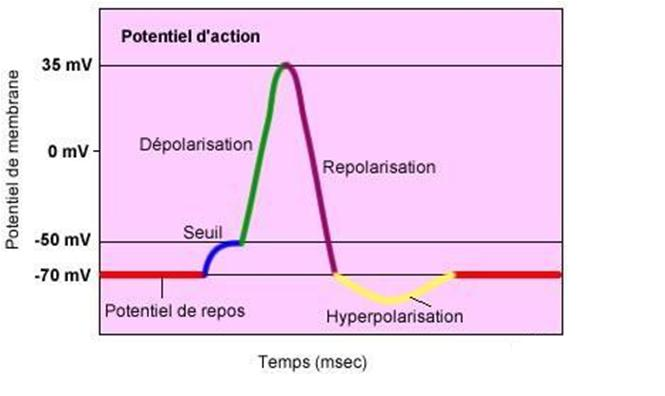
\includegraphics{imgs/2.JPG}
\caption{Potentiel de la membrane en fonction du temps lors de la production d'un potentiel d'action dans un neurone biologique \scriptsize{(http://www.cours-pharmacie.com/images/potentiel\_action.jpg)}}
\end{figure}

\section{Modèle de Hodgkin Huxley}\label{hh}
L'approche de Hodgkin et Huxley sur la question de la modélisation de neurones est une approche qui possède une grande "clarté physiologique", dans le sens où chaque composante du modèle représente une réalité biologique ou électrique descriptible dans les termes de la neurobiologie. On peut ainsi attribuer au modèle de Hodgkin-Huxley une certaine cohérence et validité par rapport aux sciences naturelles (notamment neurobiologie encore une fois). Mais voyons ça plus en détails ..
\subsection{La modélisation des canaux ioniques}
Comme nous l'avons rappelé dans \ref{rappelneuro1}, la génération de potentiels d'actions est gouvernée, au niveau moléculaire, par les dynamiques d'ouverture et de fermeture des canaux ioniques. Ces canaux peuvent être dans différents états : ouverts ou fermés, bien sûr, mais aussi actifs ou inactifs, et il est nécessaire qu'un canal soit à la fois dans l'état ouvert et actif pour que les ions puissent passer. Hodgkin-Huxley ont fait 2 hypothèses sur ces canaux ioniques dans leurs travaux, sur la base d'observation des neurones biologiques : premièrement, la génération du potentiel d'action est gouvernée par les mouvements des ions potassium et sodium, et pas des autres ions, et deuxièmement, les canaux sodiques et potassiques sont divisés en différentes composantes. Les canaux potassiques se divisent en 4 composantes équivalentes qui gouvernent l'ouverture du canal : le canal est ouvert lorsque les 4 composantes sont ouvertes. Les canaux potassiques étant de plus considérés comme toujours actifs, le passage des ions est permis lorsque ces 4 composantes sont ouvertes. Les canaux sodiques, quant à eux, se divisent en 3 composantes gouvernant l'ouverture du canal, et 1 composante gouvernant l'activation du canal. Il est nécessaire que les 3 composantes gouvernant l'ouverture soient ouvertes et que la composante gouvernant l'activation du canal soit active pour que les ions puissent passer.

On notera $n \in [0, 1]$ la probabilité qu'une composante d'un canal potassique soit ouverte, et donc $(1-n)$ est la probabilité que la composante soit fermée. On sait que l'ouverture et la fermeture de ces canaux ioniques dépend du potentiel de membrane, ainsi, on a $\alpha_n$ et $\beta_n$ des fonctions du potentiel qui définissent respectivement le passage de l'état fermé à l'état ouvert, et de l'état ouvert à l'état fermé. Si on connait la probabilité initiale $n(t_0)$ que la composante soit ouverte en $t=t_0$, on peut déduire la probabilité que la composante soit ouverte pour tout $t>t_0$. En effet, la probabilité qu'une composante soit ouverte pendant $dt$ est la probabilité qu'on soit à l'état fermé et qu'on passe de l'état fermé à l'état ouvert et qu'on soit dans l'état ouvert et qu'on ne passe pas de l'état ouvert à l'état fermé. Ainsi, 
\begin{center} $\displaystyle \frac{\dd n}{\dd t} = \alpha_n(V)(1-n) - \beta_n(V) n$ \end{center}
Et on peut réécrire cette equation sous la forme :
\begin{center} $\displaystyle \tau_n \frac{\dd n}{\dd t} = n_{\infty} - n$ \end{center}
avec $\tau_n = \frac{1}{\alpha_n+\beta_n}$ la constante de temps et $n_\infty = \frac{\alpha_n}{\alpha_n+\beta_n}$ la valeur de n à l'équilibre. \\
Etant donné qu'il est nécessaire que les quatre composantes du canal soient ouvertes pour que le canal soit lui-même "ouvert", c'est-à-dire qu'il laisse passer les ions, la probabilité que le canal soit ouvert est la probabilité que les quatre composantes soient ouvertes, soit $n^4$.

Maintenant que nous avons défini les variations de la probabilité d'ouverture des canaux potassiques, nous allons faire de même pour les canaux sodiques. La différence ici par rapport au canal potassique est qu'il faut prendre en compte, en plus de l'ouverture et de la fermeture, l'activation et l'inactivation du canal. On devra donc utiliser deux probabilité différentes : $m \in [0,1]$ la probabilité qu'une composante contrôlant l'ouverture soit ouverte (et donc $(1-m)$ est la probabilité que la composante soit fermée) et $h \in [0,1]$ la probabilité que le canal soit actif (et donc $(1-h)$ la probabilité qu'il soit inactif). Etant donné que l'activation et l'inactivation n'est contrôlée que par une seule composante, l'activation ou l'inactivation de cette composante est équivalente à l'activation ou l'inactivation du canal. On définit $\alpha_m, \beta_m, \alpha_h, \beta_h$ les fonctions du potentiel qui définissent respectivement le passage de l'état fermé à l'état ouvert d'une composante contrôlant l'ouverture, le passage de l'état ouvert à l'état fermé d'une composante contrôlant l'ouverture, le passage de l'état inactif à l'état actif du canal, le passage de l'état actif à l'état inactif du canal. Et, de la même manière que pour les canaux potassiques, on a les équations 
\begin{center} $\displaystyle \frac{\dd m}{\dd t} = \alpha_m(V)(1-m) - \beta_m(V) m$ \end{center}
\begin{center} $\displaystyle \frac{\dd h}{\dd t} = \alpha_h(V)(1-h) - \beta_h(V) h$ \end{center}
Que l'on peut réécrire comme ceci :
\begin{center} $\displaystyle \tau_m \frac{\dd m}{\dd t} = m_{\infty} - m$ \end{center}
\begin{center} $\displaystyle \tau_h \frac{\dd h}{\dd t} = h_{\infty} - h$ \end{center}
avec encore une fois $\tau_m = \frac{1}{\alpha_m+\beta_m},~\tau_h = \frac{1}{\alpha_h+\beta_h} $ les constantes de temps et \\$m_\infty = \frac{\alpha_m}{\alpha_m+\beta_m},~h_\infty = \frac{\alpha_h}{\alpha_h+\beta_h}$ les valeurs de m et h à l'équilibre. \\
Ici, il est nécessaire que le canal soit actif et que les trois composantes controlant l'ouverture soient ouvertes pour que le canal laisse passer les ions, ainsi la probabilité que le canal laisse passer les ions est $m^3h$.

En plus des ces équations qui permettent de connaitre la probabilité qu'un canal soit ouvert au temps t, on va également définir les conductances d'un canal lorsqu'il est ouvert et le potentiel d'équilibre associé à chaque ion. On notera $\overline{g_{Na}}$ et $\overline{g_K}$ les conductances associées respectivement aux ions sodium et potassium, et $V_{Na}$ et $V_K$ les potentiels d'équilibre donné par la formule de Nernst pour respectivement les ions sodium et potassium.

Pour finir, Hodgkin et Huxley ont également introduit dans leur modèle un "courant de fuite", c'est-à-dire un courant qui modélise l'impact de tous les échanges d'ions qui ne sont pas gouvernés par les canaux sodium et potassium. On va donc définir en plus $\overline{g_L}$ et $V_L$ respectivement la conductance et le potentiel d'équilibre associée à ce courant de fuite.

\pagebreak
\subsection{L'équation du potentiel de membrane} \label{HHEQPOT}
Il est possible de représenter un neurone dans le modèle de Hodgkin-Huxley comme un circuit électrique (voir figure \ref{HHFIG}). Dans cette représentation, on peut assimiler le condensateur à la bicouche lipidique isolante de la membrane, la résistance aux passages des ions à travers la membrane, et la pile aux gradients de concentration. Grace à cette représentation, il est plus facile d'expliquer l'équation représentant les variations du potentiel de membrane du neurone. On va ici en faire une explication intuitive en se basant sur des grands principes issus des sciences physiques :\\
\begin{itemize}
\item La loi d'Ohm énonce que l'on peut relier la valeur d'une résistance en ohms (notée R), la tension aux bornes de la résistance (notée V) et le courant qui traverse la résistance (noté I) par la relation : \begin{center}$ V = RI $\end{center}
\item La loi des nœuds de Kirchhoff stipule que "la somme algébrique des intensités des courants qui entrent par un nœud est égale à la somme algébrique des intensités des courants qui en sortent"
\item Un condensateur est constitué de deux armatures séparées par un isolant. La loi du condensateur est : \begin{center} $Q = CV$ \end{center} avec Q la charge du condensateur, C la capacité du condensateur et V la tension aux bornes du condensateur. \\ De plus, la dérivée de la charge par rapport au temps est l'intensité du courant, c'est-à-dire \begin{center}$\displaystyle \frac{\dd Q}{\dd t} = I $ \end{center}
\item On définit la conductance g associée à une résistance comme l'inverse de la valeur de la résistance \begin{center} $g = \displaystyle \frac{1}{R}$ \end{center}
\end{itemize}

\clearpage
\begin{figure}[!h]
\centering
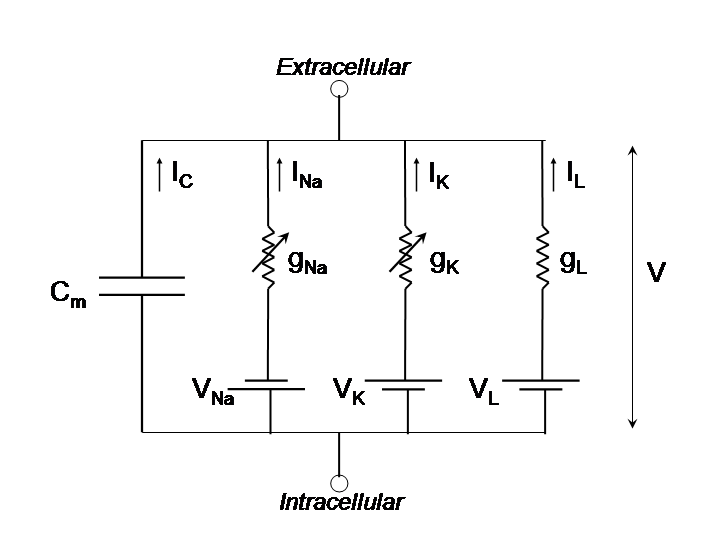
\includegraphics[scale=0.5]{imgs/3.png}
\caption{Représentation du modèle de Hodgkin-Huxley sous forme d'un circuit électrique (\scriptsize{https://thephysicsdomain.wordpress.com/2013/03/28/047-hodgkin-huxley-hysteria/})}
\label{HHFIG}
\end{figure}

Dans ce paragraphe on se reportera à la figure \ref{HHFIG}. On va noter $I_{app}$ le courant appliquée sur la cellule de l'extérieur. De la loi de Kirchhoff, on peut déduire que \begin{equation} I_C+I_{Na}+I_K+I_L-I_{app} = 0 \label{Toteq}\end{equation} 

De la définition d'un condensateur, on a \begin{equation} I_C = \frac{\dd Q}{\dd t} = C\frac{\dd V}{\dd t} \label{Ceq}\end{equation} 

De plus, par la loi d'Ohm, on peut noter \begin{equation}I_{Na} = \frac{V^*}{R^*} = g^*V^* \nonumber\end{equation} avec $V^*$ la tension aux bornes de la résistance et $g^*$ la conductance associée aux courant sodique.\\La tension aux bornes de la résistance $V^*$ est atténuée par la présence de la pile, et on a ainsi $V^* = V - V_{Na}$. Quant à la conductance associée aux courants sodiques, elle dépend de la conductance maximale $\overline{g_{Na}}$ et de la proportion de canaux sodiques laissant passer les ions (c'est-à-dire ici approximativement de la probabilité qu'un canal sodique laisse passer les ions, puisqu'on considère que le nombre de canaux est très grand), et on a $g^* = \overline{g_{Na}}m^3h$. Et donc, \begin{equation}I_{Na} = \overline{g_{Na}}m^3h(V-V_{Na}) \label{Naeq}\end{equation}
Et, par le même raisonnement, 
\begin{equation}I_{K} = \overline{g_{K}}n^4(V-V_{K}) \label{Keq}\end{equation}
Et
\begin{equation}I_{L} = \overline{g_{L}}(V-V_{L}) \label{Leq}\end{equation}

En introduisant \ref{Ceq}, \ref{Naeq}, \ref{Keq} et \ref{Leq} dans \ref{Toteq}, on trouve une équation décrivant l'évolution du potentiel membranaire : \begin{center}$\displaystyle C\frac{\dd V}{\dd t} = -\overline{g_K}n^4(V-V_K)- \overline{g_{Na}}m^3h(V-V_{Na})-\overline{g_L}(V-V_L)+I_{app}$ \end{center}
A partir de cette dernière équation et des équations décrivant les comportements des canaux ioniques, on peut donner le système d'équations de Hodgkin-Huxley dans son entièreté : \\ 
\setcounter{equation}{0}\begin{empheq}[left=\empheqlbrace]{gather} \displaystyle C\frac{\dd V}{\dd t} = -\overline{g_K}n^4(V-V_K)- \overline{g_{Na}}m^3h(V-V_{Na})-\overline{g_L}(V-V_L)+I_{app}\\ \displaystyle \frac{\dd n}{\dd t} = \alpha_n(V)(1-n) - \beta_n(V) n\\ \displaystyle \frac{\dd m}{\dd t} = \alpha_m(V)(1-m) - \beta_m(V) m \\ \displaystyle \frac{\dd h}{\dd t} = \alpha_h(V)(1-h) - \beta_h(V) h\end{empheq}




\subsection{Simulation avec SNN.single et explication des dynamiques}

On va simuler le modèle de Hodgkin-Huxley à l'aide de l'outil informatique que nous avons mis en place.

Pour simuler numériquement le modèle, il faut avoir des valeurs pour $C_M$, les conductances $\overline{g_X}$, les potentiels d'équilibre $V_X$, et les fonctions $\alpha_X$ et $\beta_X$.
En tentant de rapprocher les comportements du modèle de données physiologiques récoltées à l'aide de la technique de patch-clamp (originellement dans les travaux de Hodgkin-Huxley sur un axone de calamar, ayant la particularité d'être très gros et donc très facile à étudier), on trouve les valeurs pour les paramètres : \\\\
$ C_M = 1,~ \overline{g_K} = 36,~ \overline{g_{Na}} = 120,~ \overline{g_L} = 0.3,~ V_K = -77,~ V_{Na} = 50,~ V_L = -54.4,\\\\
\alpha_n(V) =\frac{ 0.01(-V-55)}{\e^{\frac{-V-55}{10}}-1},~ \beta_n=0.125e^{\frac{-V-65}{80}}\\\\
\alpha_n(V) =\frac{ 0.1(-V-40)}{\e^{\frac{-V-40}{10}}-1},~ \beta_n=4e^{\frac{-V-65}{18}}\\\\
\alpha_n(V) =0.07e^{\frac{-V-65}{20}},~ \beta_n=\frac{1}{1+e^{\frac{-V-35}{10}}}$
\clearpage

\begin{lstlisting}[caption = {Hodgkin-Huxley : Définition du modèle}]
from .core import Variable, Model
V = Variable(name='V', init_value=-60, unit='mV',
ddt='(1/Cm)*(-gk*n**4*(V-Vk)-gna*m**3*h*(V-Vna)-gl*(V-Vl)+Iapp)')
n = Variable(name='n', ddt='alpha_n*(1-n)-beta_n*n', init_value=1/3)
m = Variable(name='m', ddt='alpha_m*(1-m)-beta_m*m', init_value=0)
h = Variable(name='h', ddt='alpha_h*(1-h)-beta_h*h', init_value=2/3)
HH = Model(V, n, m, h, Cm=1, gk=36, gna=120, 
gl=0.3, Vk=-77, Vna=50, Vl=-54.4, 
alpha_n='0.01*(-V-55)/(exp((-V-55)/10) -1)', 
beta_n='0.125*exp((-V-65)/80)',
alpha_m='0.1*(-V-40)/(exp((-V-40)/10) -1)', 
beta_m='4*exp((-V-65)/18)',
alpha_h='0.07*exp((-V-65)/20)',
beta_h='1/(1+exp((-V-36)/10))', 
Iapp=0)
\end{lstlisting}

\begin{lstlisting}[caption = {Hodgkin-Huxley : Simulation du modèle pour $I_{app} = 5$}]
from snn.single.usual_models import HH as hh
import matplotlib.pyplot as plt

# Define Input current
hh['Iapp'] = 5
# Runge-Kutta method for numerical simulation
hh.method = 'rk4'

# Since we are plotting multiple things, it's better to simulate the
# model only one time, and then feed the results to the plot method
T, dt = 100, 0.01
history, _ = hh.simulation(T, dt)

# Plot the input current and the membrane 
# potential evolution throught time
hh.plot(T, dt, keep=['V', 'Iapp'], history=history)

# Print m, n, h evolution when the membrane potentiel changes
hh.phase_portrait(T, dt, 'V', 'm', history=history)
hh.phase_portrait(T, dt, 'V', 'n', history=history)
hh.phase_portrait(T, dt, 'V', 'h', history=history)

plt.show()
\end{lstlisting}



\begin{figure}[!h]
\centering
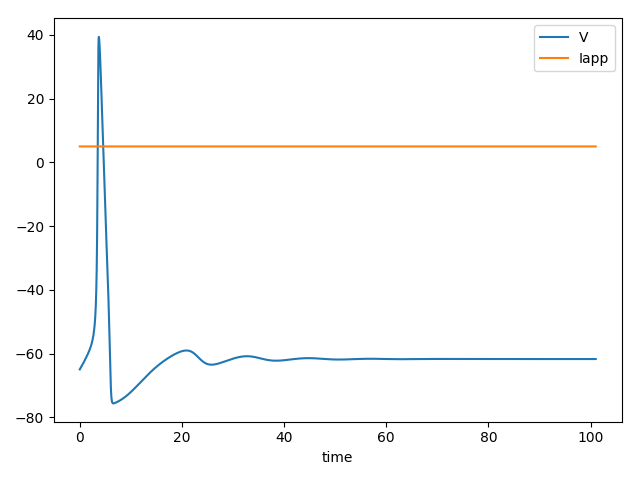
\includegraphics[scale=0.5]{imgs/hh11.png}
\caption{Hodgkin-Huxley : Evolution du potentiel de membrane au cours du temps pour $I_{app} = 5$}
\label{hh11}
\end{figure}

\begin{figure}[!h]
\begin{minipage}[l]{.3\linewidth}
\centering
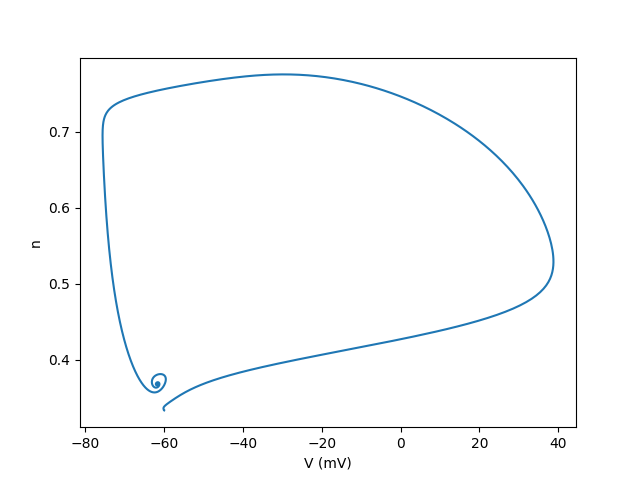
\includegraphics[scale=0.35]{imgs/hh12.png}
\end{minipage}\hfill
\begin{minipage}[l]{.3\linewidth}
\centering
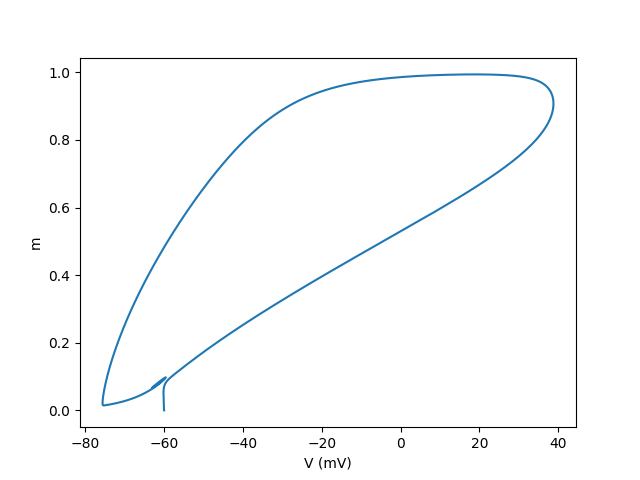
\includegraphics[scale=0.35]{imgs/hh13.png}
\end{minipage}\hfill
\begin{minipage}[l]{.3\linewidth}
\centering
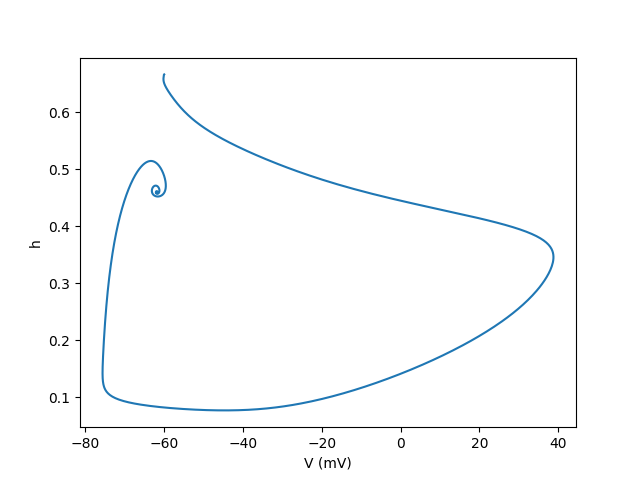
\includegraphics[scale=0.35]{imgs/hh14.png}
\end{minipage}\hfill
\caption{Hodgkin-Huxley : n, m et h en fonction de V pour $I_{app} = 5$}
\label{hh1234}
\end{figure}

\clearpage

\begin{lstlisting}[caption = {Hodgkin-Huxley : Simulation du modèle pour $I_{app} = 10$}]
hh['Iapp'] = 10
T, dt = 100, 0.01
\end{lstlisting}

\begin{figure}[!h]
\centering
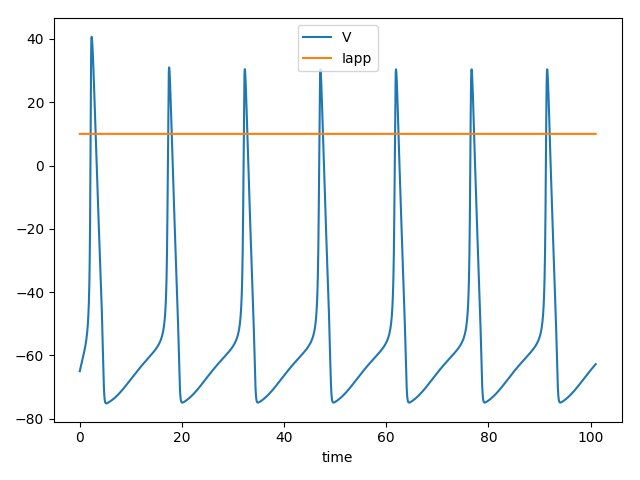
\includegraphics[scale=0.4]{imgs/hh21.png}
\caption{Hodgkin-Huxley : Evolution du potentiel de membrane au cours du temps pour $I_{app} = 10$}
\label{hh21}
\end{figure}

\begin{figure}[!h]
\begin{minipage}[l]{.3\linewidth}
\centering
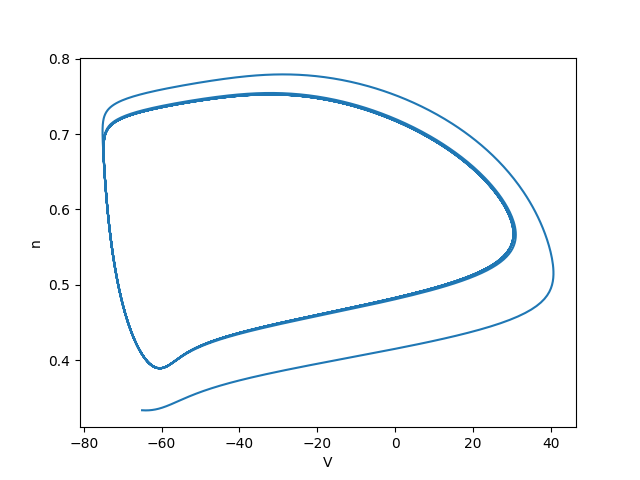
\includegraphics[scale=0.35]{imgs/hh22.png}
\end{minipage}\hfill
\begin{minipage}[l]{.3\linewidth}
\centering
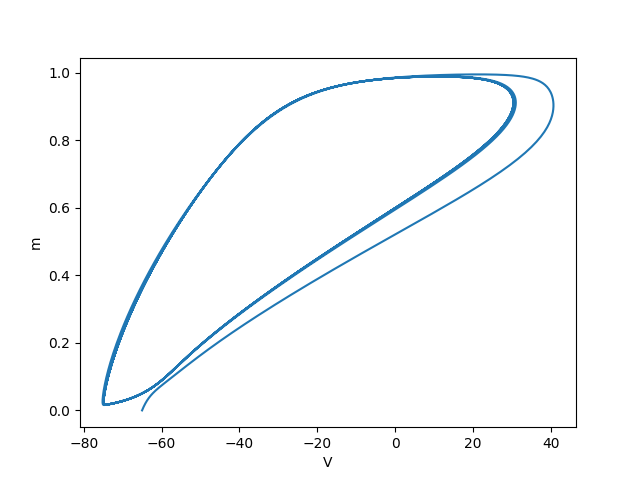
\includegraphics[scale=0.35]{imgs/hh23.png}
\end{minipage}\hfill
\begin{minipage}[l]{.3\linewidth}
\centering
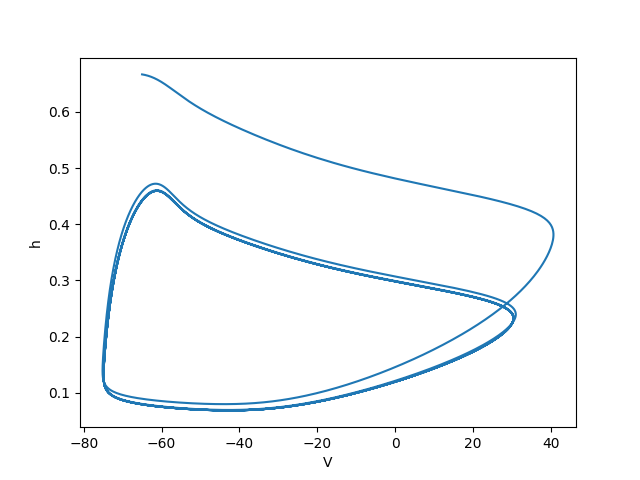
\includegraphics[scale=0.35]{imgs/hh24.png}
\end{minipage}\hfill
\caption{Hodgkin-Huxley : n, m et h en fonction de V pour $I_{app} = 10$}
\label{hh2234}
\end{figure}

Dans \ref{hh11}, on peut voir que le modèle est bien capable de produire un potentiel d'action, en tout cas le comportement de la variable V représentant le potentiel de membrane a un comportement similaire aux potentiel de membrane \textit{in vivo}. Le courant appliqué, qui est constant égal à 5, est suffisant pour provoquer un potentiel d'action mais insuffisant pour en provoquer un deuxième. Au contraire, dans \ref{hh21}, le courant constant égal à 10 est suffisant pour provoquer un train de potentiel d'action, à partir du deuxième potentiel d'action, on a un comportement périodique du système, qui va continuer de générer des potentiels d'action si le courant appliqué reste constant. Cela peut également se voir sur les représentations de m, n et h en fonction de V. Lorsqu'il n'y a qu'un seul potentiel d'action puis une convergence vers un état stable, on peut voir dans \ref{hh1234} la présence d'un équilibre attracteur pour m, n et h, ce qui signifie que l'état du système va se stabiliser. Au contraire, lorsqu'on a une génération périodique de potentiel d'action comme dans \ref{hh2234}, on voit bien que le comportement de m, n et h est cyclique et qu'il n'y a pas d'équilibre attracteur.

\begin{lstlisting}[caption = {Hodgkin-Huxley : Simulation du modèle pour $I_{app}$ définie par morceau}]
hh['Iapp'] = '5 if 200<t<400 else 10 if 600<t<800 else 0'
T, dt = 1000, 0.01
\end{lstlisting}

\begin{figure}[!h]
\centering
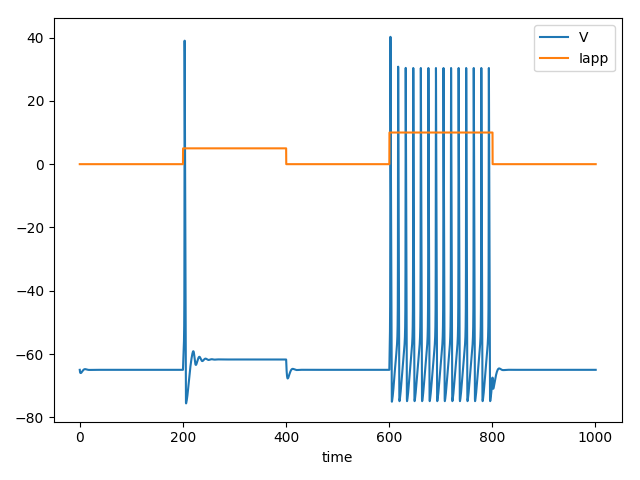
\includegraphics[scale=0.8]{imgs/hh31.png}
\caption{Hodgkin-Huxley : Evolution du potentiel de membrane au cours du temps pour $I_{app}$ définie par morceau}
\label{hh31}
\end{figure}

\clearpage
\begin{lstlisting}[caption = {Hodgkin-Huxley : Simulation du modèle pour $I_{app} = 5\cos(\frac{t}{10})+\epsilon(\frac12)$}]
hh['Iapp'] = '5*math.cos(t/10) + rd.expovariate(0.5)'
T, dt = 100, 0.01
\end{lstlisting}

\begin{figure}[!h]
\centering
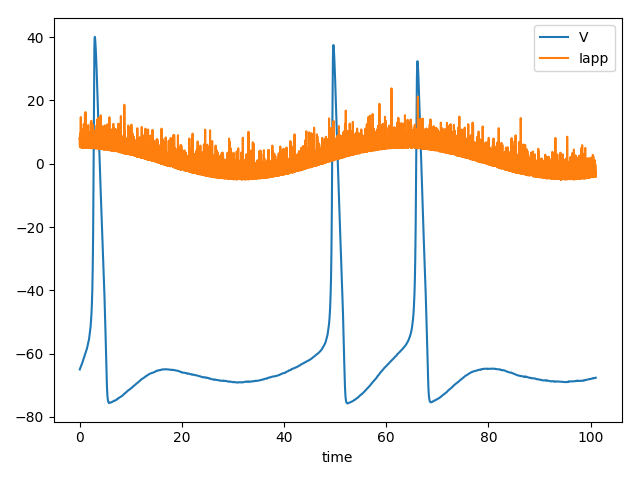
\includegraphics[scale=0.8]{imgs/hh41.png}
\caption{Hodgkin-Huxley : Evolution du potentiel de membrane au cours du temps pour $I_{app} = 5\cos(\frac{t}{10})+\epsilon(\frac12)$}
\label{hh41}
\end{figure}

\clearpage 
\begin{lstlisting}[caption = {Hodgkin-Huxley : Evolution de m, n et h lors d'un potentiel d'action}]
hh['Iapp'] = 10
T, dt = 12, 0.01
hh.plot(T, dt, keep=['m', 'n', 'h'], #subplotform='31', 
history=history)
\end{lstlisting}

\begin{figure}[!h]
\centering
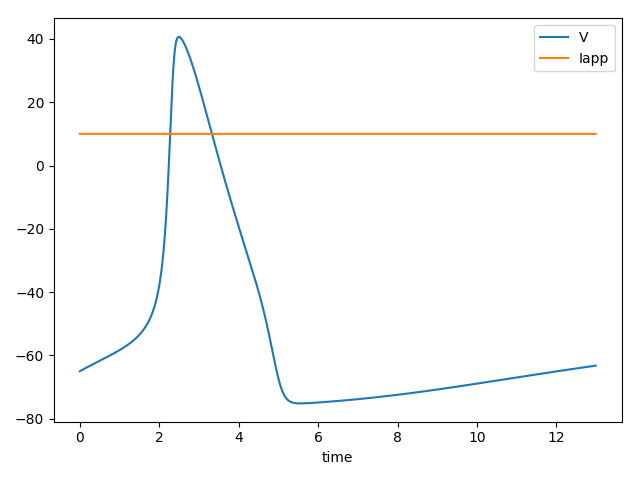
\includegraphics[scale=0.5]{imgs/hh51.png}
\caption{Hodgkin-Huxley : Evolution du potentiel de membrane lors d'un potentiel d'action}
\label{hh51}
\end{figure}

\begin{figure}[!h]
\centering
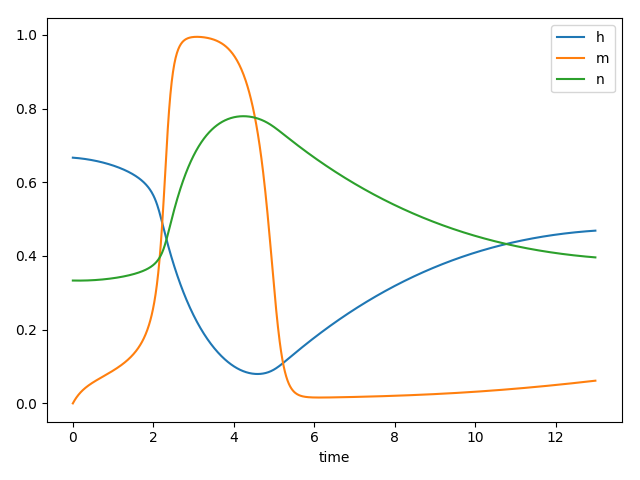
\includegraphics[scale=0.5]{imgs/hh52.png}
\caption{Hodgkin-Huxley : Evolution des paramètres m, n et h lors de la génération d'un potentiel d'action}
\label{hh52}
\end{figure}

\clearpage

\begin{lstlisting}[caption = {Hodgkin-Huxley : Constantes de temps et états à l'équilibre}]
hh['Iapp'] = 10
T, dt = 12, 0.01

#Plotting time constant
plt.figure()
plt.plot(history['V'], 1/(history['alpha_n']+history['beta_n']),
label='\u03C4_n')
plt.plot(history['V'], 1/(history['alpha_m']+history['beta_m']),
label='\u03C4_m')
plt.plot(history['V'], 1/(history['alpha_h']+history['beta_h']),
label='\u03C4_h')
plt.legend()

#Plotting equilibrium state
plt.figure()
plt.plot(history['V'],
history['alpha_n']/(history['alpha_n']+history['beta_n']),
label='n_\u221E')
plt.plot(history['V'],
history['alpha_m']/(history['alpha_m']+history['beta_m']),
label='m_\u221E')
plt.plot(history['V'],
history['alpha_h']/(history['alpha_h']+history['beta_h']),
label='h_\u221E')
plt.legend()

plt.show()
\end{lstlisting}

\begin{figure}[!h]
\centering
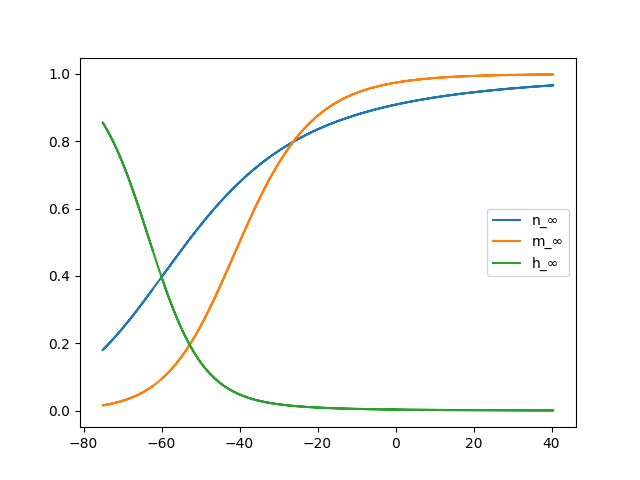
\includegraphics[scale=0.65]{imgs/hhinfty.png}
\caption{Hodgkin-Huxley : Evolution des paramètres $n_\infty$, $m_\infty$ et $h_\infty$ lors de la génération d'un potentiel d'action}
\label{hhinfty}
\end{figure}

\begin{figure}[!h]
\centering
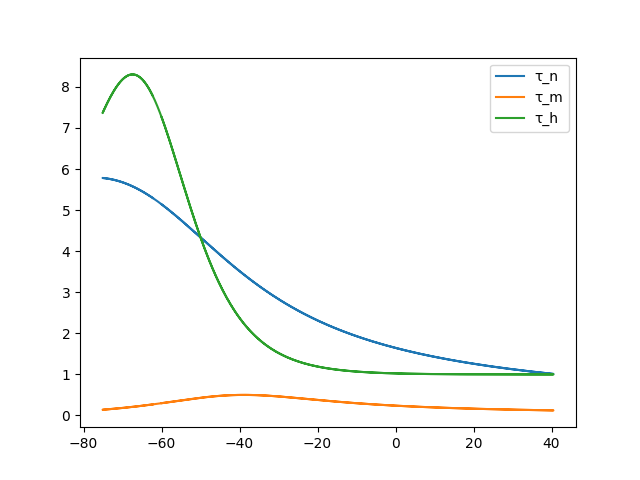
\includegraphics[scale=0.65]{imgs/hhtime.png}
\caption{Hodgkin-Huxley : Evolution des paramètres $\tau_n$, $\tau_m$, $\tau_h$ lors de la génération d'un potentiel d'action}
\label{hhtime}
\end{figure}

\clearpage
\textbf{Explication des dynamiques à partir des constantes de temps et des valeurs à l'équilibre}\\
De \ref{hhinfty}, on peut tirer le fait que n et m sont croissants par rapport au potentiel, tandis que h est décroissant par rapport au potentiel. Ainsi, les canaux potassiques vont avoir une probabilité de laisser passer les ions (qui est, rappelons-le, exprimée par $n^4$) de plus en plus grande plus le potentiel augmente, tandis que pour les canaux sodiques, leur probabilité de laisser passer les ions (qui est $m^3h$) va d'abord augmenter quand le potentiel augmente (dû au fait que m est croissante par rapport au potentiel), puis, à partir d'un certain seuil, diminuer quand le potentiel augmente (dû au fait que h est décroissante par rapport au potentiel).\\
Les constantes de temps, qui gouvernent le temps que met le système à atteindre les valeurs à l'équilibre, sont également intéressantes à étudier pour comprendre les dynamiques à l'œuvre. On peut voir dans \ref{hhtime}, que m (ouverture des canaux sodiques), atteint très rapidement sont état d'équilibre, tandis que n (ouverture des canaux potassiques) et h (activation des canaux sodiques) l'atteignent plus lentement.\\
Ainsi, lorsque la membrane est dépolarisée, la variable m va augmenter (vers son état d'équilibre $m_\infty$) rapidement (les canaux sodiques vont s'ouvrir rapidement), ce qui va en retour augmenter la dépolarisation de la cellule (le potentiel de membrane va tendre vers $V_{Na}$), et m va de nouveau augmenter, etc. Avec un délai dû aux dynamiques (c'est-à-dire ici au temps d'atteinte de la valeur d'équilibre) plus lentes de h et n, on va observer que h va diminuer (tendre vers sa valeur d’équilibre $h_\infty$) (les canaux sodiques vont être désactivés), et de plus, n va augmenter (tendre vers sa valeur d'équilibre $n_\infty$) (les canaux potassiques vont s'ouvrir), ce qui aura pour effet de repolarisée la cellule (le potentiel de membrane va tendre vers $V_{K}$). La période réfractaire, c'est-à-dire l'hyperpolarisation de la membrane peut s'expliquer par le délai dans le retour à un état d'équilibre de la variable n (les canaux potassiques se referment avec un délai).


\section{Raffiner Hodgkin-Huxley}
\subsection{Les deux approches possibles face à Hodgkin-Huxley}
Les travaux de Hodgkin et Huxley abordé en \ref{hh} ont véritablement révolutionné le domaine de la modélisation de neurones, et depuis, une grande partie des travaux en modélisation de neurones s'appuient sur ceux de Hodgkin et Huxley. Les scientifiques s'intéressant à la modélisation de neurones ont pu avoir deux grandes approches (ces deux grandes approches pouvant s'étendre à tous les travaux en modélisation de neurones, et pas seulement à ceux se basant sur le modèle de Hodgkin et Huxley) : 
\begin{enumerate} \item \textbf{Complexifier Hodgkin-Huxley : Reproduire le plus fidèlement possible un neurone ou un réseau de neurone sans se soucier de la complexité du modèle}, ce qui donne un modèle plus précis, plus proche de la réalité, mais difficilement manipulable et compréhensible, et dont la simulation est couteuse (en temps). On retrouve dans cette catégorie la plupart des modèles dit "physiologiques", c'est-à-dire les modèles qui s'inspirent du fonctionnement biologique du système nerveux et tentent de le formaliser. 
\item \textbf{Simplifier Hodgkin-Huxley : Faire un compromis entre le réalisme du modèle et sa complexité}, ce qui donne des modèles moins précis et moins proche de la réalité, mais plus facilement manipulable, compréhensible et dont la simulation est rapide. On retrouve dans cette catégorie la plupart des modèles dit "phénoménologiques", c'est-à-dire les modèles qui, sans la contrainte de s'inspirer du biologique, tentent de reproduire le fonctionnement du système nerveux en termes de données quantitatives "de plus haut niveau", comme par exemple le potentiel de membrane d'un neurone. \end{enumerate}
Un modèle de neurone théorique parfait devrait posséder les qualités des deux approches sans posséder leurs défauts ... mais cela semble pour l'instant impossible. Le réalisme passe par la complexité du modèle, et la complexité du modèle entraine que la simulation informatique et que l'explication mathématique seront couteuses. Ainsi, lorsque l'on doit choisir un modèle de neurone, on doit le faire dans objectif précis, et il est important de bien comprendre quelles sont les caractéristiques du modèle importantes pour réaliser notre objectif. Dans le cas de ce travail, nous allons par la suite vouloir réaliser des simulations de réseaux de grandes tailles de manière rapide, répétable. C'est ainsi, et c'est un choix de notre part, que nous allons ici plutôt nous intéresser aux modèles simples, venant de l'approche 2., pour leur simplicité et rapidité de simulation. 


\subsection{De Hodgkin-Huxley à Fitzhugh-Nagumo}
Nous allons maintenant nous intéresser à l'approche de Fitzhugh et Nagumo dans la réduction de la complexité du modèle de Hodgkin-Huxley. Cette approche de Fitzhugh-Nagumo est basée sur deux approximations du modèle de Hodgkin-Huxley : 
\begin{itemize}
\item $m_{\infty}(V) \simeq m(t)$, c'est-à-dire que $m$ peut être en tout temps approximé par sa valeur à l'équilibre. Cette approximation est justifiée par le fait que les variations de $m$ sont très rapides, en tout cas, comparées à celle de $h$ et $n$ (cela peut se voir sur la figure \ref{hhtime} des constantes de temps). Ainsi, $\frac{\dd m}{\dd t} = 0$, et l'équation décrivant l'évolution de m dans le temps dans le modèle de Hodgkin-Huxley n'a plus de raison d'être.
\item $h_\infty + n_\infty \simeq 0.85$, c'est-à-dire que la somme des valeurs à l'équilibre de $h$ et $n$ est constante (voir figure \ref{hhnplush}). Fitzhugh et Nagumo ont ensuite élargie cette approximation à $n(t)$ et $h(t)$, c'est-à-dire que $\exists a,b \in \mathbb{R} \text{ tq }, h(t) + an(t) = b$. On peut ainsi définir $w = b-h(t) = an(t)$, et on a $w$ qui décrit ainsi en même temps l'évolution des variables $h$ et $n$, et on a $\displaystyle \frac{\dd w}{\dd t} = a\frac{\dd n}{\dd t} = \frac{an_\infty -an}{\tau_n} = \frac{w_\infty-w}{\tau_w} \text{ avec } w_\infty=an_\infty, \tau_w = \tau_n$. Cette nouvelle variable w représente le rétablissement de la membrane. \end{itemize}

\begin{lstlisting}[caption = {Hodgkin-Huxley : Somme de n et h}]
from snn.single.usual_models import HH as hh
import matplotlib.pyplot as plt

plt.figure() ; plt.xlabel('time') ; plt.ylabel('n+h')
for I in [0, 5, 10]:
hh['Iapp'] = I
history, _ = hh.simulation(100, 0.1)
plt.plot(history['t'], history['n'] + history['h'], 
label='n+h in HH-model with current %s' % I)
plt.legend()
plt.show()
\end{lstlisting}

\begin{figure}[!h]
\centering
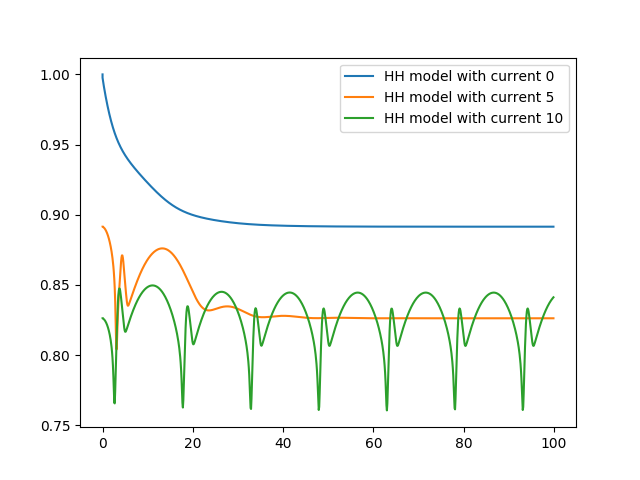
\includegraphics[scale=0.5]{imgs/hhnplush.png}
\caption{Somme de n et h dans le modèle de Hodgkin-Huxley}
\label{hhnplush}
\end{figure}

On peut alors réécrire le modèle de Hodgkin-Huxley avec ces approximations :
\setcounter{equation}{0}\begin{empheq}[left=\empheqlbrace]{gather} \displaystyle C\frac{\dd V}{\dd t} = -\overline{g}_K(\frac{w}{a})^4(V-V_K)- \overline{g}_{Na}m_\infty^3(b-w)(V-V_{Na})-\overline{g}_L(V-V_L)+I\nonumber \\ \displaystyle \frac{\dd w}{\dd t} = \frac{w_\infty-w}{\tau_w} \nonumber \end{empheq}
En traçant les isoclines de ce modèle, on se rend compte qu'elles semblent être approximables, pour la V-isocline, par une fonction polynomiale de degré 3, et pour la W-isocline, par une droite.\\
On peut donc approximer ce modèle par :
\setcounter{equation}{0}\begin{empheq}[left=\empheqlbrace]{gather} \displaystyle C \frac{\dd V}{\dd t} = \alpha V^3 +\beta V^2 + \gamma V + \delta - w + I \nonumber\\ \displaystyle \tau\frac{\dd w}{\dd t} = V+a-bw \nonumber \end{empheq}
Et en cherchant à faire coïncider les comportements de ce modèle avec ceux des neurones biologiques (ou ceux du modèle de Hodgkin-Huxley), on trouve les valeurs de $\alpha, \beta, \gamma, \delta, a, b, C$ et $\tau$, et on peut ainsi écrire le modèle de Fitzhugh-Nagumo dans sa forme la plus courante :
\setcounter{equation}{0}\begin{empheq}[left=\empheqlbrace]{gather} \displaystyle \frac{\dd V}{\dd t} = V - \frac{V^3}{3} - w + I \\ \displaystyle \frac{\dd w}{\dd t} = 0.08(V+0.7-0.8w) \end{empheq}
On a ainsi un système de dimension 2 qui conserve les propriétés fondamentales en termes de dynamiques du système de dimension 4 de Hodgkin-Huxley. Un des avantages que cela comporte est que les dynamiques du système sont entièrement explicables par l'analyse du plan de phase du modèle (voir figure \ref{FNPDP}). J'encourage vivement, pour ceux que cela intéresse, à utiliser la fonction "plan de phase interactif" de la bibliothèque SNN pour mieux comprendre les dynamiques à l'œuvre. Une très bonne analyse du plan de phase de ce modèle a également été faite dans un article accessible sur ScholarPedia à l'adresse \url{http://www.scholarpedia.org/article/FitzHugh-Nagumo_model}.

\begin{lstlisting}[caption = {Fitzhugh-Nagumo : Définition du modèle}]
from .core import Variable, Model
v = Variable(name='v', ddt='v-(1/3)*v**3-w+I', init_value=0)
w = Variable(name='w', ddt='(1/tau)*(v+a-b*w)', init_value=0)
FHN = Model(v, w, a=0.7, b=0.8, tau=12.5, I=0.5)
\end{lstlisting}
\begin{lstlisting}[caption = {Fitzhugh-Nagumo : Plan de phase}]
from snn.single.usual_models import FHN as fhn
import matplotlib.pyplot as plt
fhn.phase_plan(('v', -2.5, 2), ('w', -1, 1))
plt.show()
\end{lstlisting}

\begin{figure}[!h]
\centering
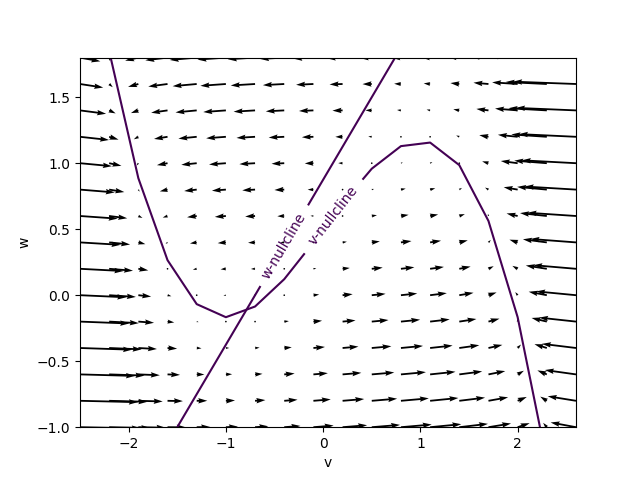
\includegraphics[scale=0.7]{imgs/FNPDP.png}
\caption{Fitzhugh-Nagumo : Plan de phase}
\label{FNPDP}
\end{figure}

\clearpage
\begin{lstlisting}[caption = {Comparaison des comportements des modèles de Fitzhugh-Nagumo et Hodgkin-Huxley}]
from snn.single.usual_models import FHN as fhn, HH as hh
import matplotlib.pyplot as plt

fhn['tau'] = 5
for hh_I, fhn_I in zip([0, 5, 10], [-0.25, 0.25, 0.5]):
plt.figure()
hh['Iapp'] = hh_I ; fhn['I'] = fhn_I
fhn_history, _ = fhn.simulation(100, 0.1)
hh_history, _ = hh.simulation(100, 0.1)
plt.subplot('121') ; plt.ylim(-2, 2) 
plt.title('Fitzhugh-Nagumo model')
plt.plot(fhn_history['t'], fhn_history['v'], '-r')
plt.subplot('122') ; plt.ylim(-80, 40) 
plt.title('Hodgkin-Huxley model')
plt.plot(hh_history['t'], hh_history['V'], '-b') 
plt.show()
\end{lstlisting}

\begin{figure}[!h]
\centering
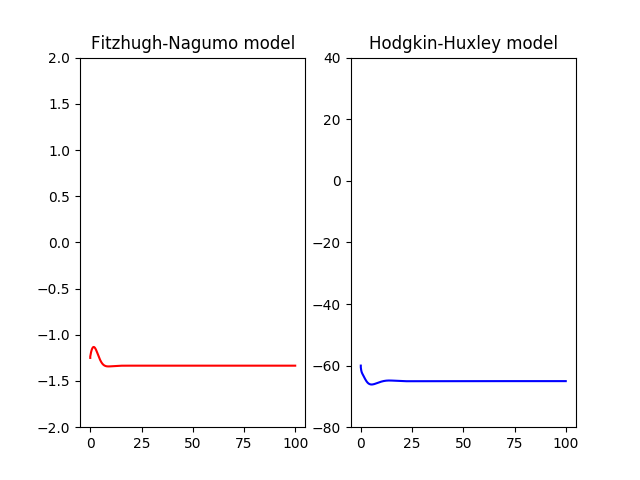
\includegraphics[scale=0.5]{imgs/hhfhnfaible.png}
\caption{Modèles de Hodgkin-Huxley et Fitzhugh-Nagumo pour des courants faibles}
\label{hhfhnfaible}
\end{figure}

\clearpage
\begin{figure}[!h]
\centering
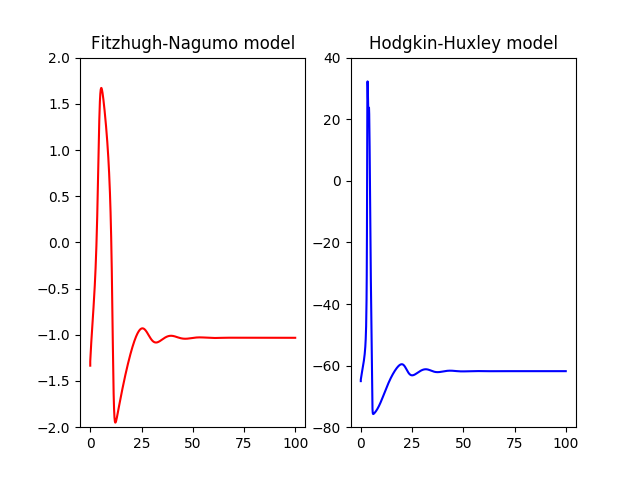
\includegraphics[scale=0.5]{imgs/hhfhnmoyen.png}
\caption{Modèles de Hodgkin-Huxley et Fitzhugh-Nagumo pour des courants moyens}
\label{hhfhnmoyen}
\end{figure}

\begin{figure}[!h]
\centering
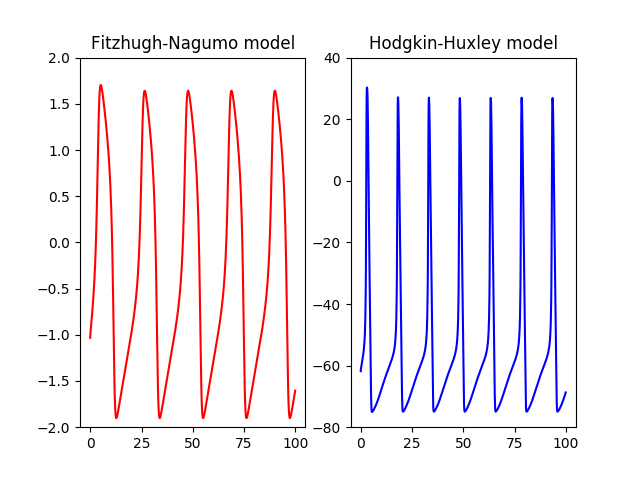
\includegraphics[scale=0.5]{imgs/hhfhnfort.png}
\caption{Modèles de Hodgkin-Huxley et Fitzhugh-Nagumo pour des courants forts}
\label{hhfhnfort}
\end{figure}

\subsection{De Fitzhugh-Nagumo à Izhikievich, et démonstration de la puissance du modèle de Izhikievich}

\begin{figure}[!h]
\centering
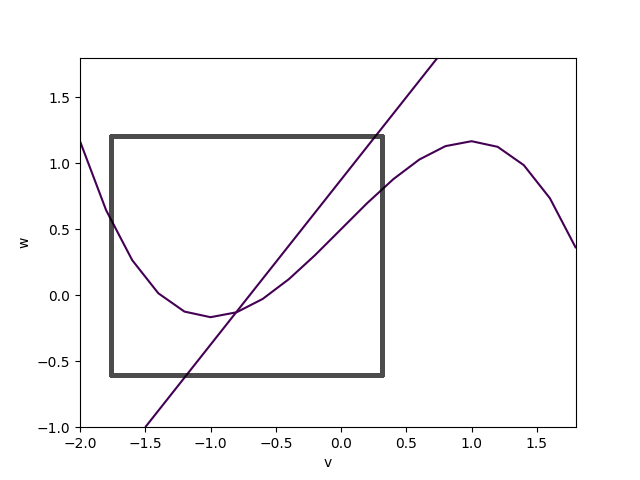
\includegraphics[scale=0.5]{imgs/fhntoiz.png}
\caption{Remarque sur le plan de phase de Fitzhugh-Nagumo}
\label{fhntoiz}
\end{figure}

A partir d'une analyse du plan de phase du modèle de Fitzhugh-Nagumo, on peut remarquer que, dans la région du plan de phase responsable de la génération des potentiels d'actions, la V-isocline peut s'approximer par une parabole, c'est-à-dire la courbe d'une fonction polynomiale de degré 2 (partie entourée sur \ref{fhntoiz}). On peut donc construire un nouveau modèle à partir de celui de Fitzhugh-Nagumo et de cette remarque, en remplaçant la V-isocline dans le modèle de Fitzhugh-Nagumo par une fonction polynomiale de degré 2 :
\setcounter{equation}{0}
\begin{empheq}[left=\empheqlbrace]{gather}
\frac{\mathrm{d}v}{\mathrm{d}t} = \alpha v^2 + \beta v + \gamma -u + I \nonumber \\
\frac{\mathrm{d}u}{\mathrm{d}t} = a(bv-u) \nonumber
\end{empheq}

En essayant de faire coïncider les comportements du modèle avec ceux des neurones biologiques, on trouve les valeurs de $\alpha = 0.04, ~\beta = 5,~ \gamma = 140$. On peut donc réecrire le modèle : \begin{empheq}[left=\empheqlbrace]{gather}
\frac{\mathrm{d}v}{\mathrm{d}t} = 0.04v^2 + 5v + 140 -u + I \\
\frac{\mathrm{d}u}{\mathrm{d}t} = a(bv-u) 
\end{empheq}

Avec ce modèle, il devient nécessaire d'introduire une règle spéciale pour les neurones qui viennent de produire un potentiel d'action. 
\begin{center} Si $ v \ge 30 mV$, alors : \end{center}
\begin{empheq}[left=\empheqlbrace]{equation}
\begin{split}
v \leftarrow c \\
u \leftarrow u + d
\end{split}
\end{empheq}

Comme dans le modèle de Fitzhugh-Nagumo, la variable $v$ symbolise le potentiel de membrane, et $u$ est une variable symbolisant le rétablissement de la membrane.\\
Les paramètres du modèle sont :
\begin{itemize}
\item $a$, qui contrôle le temps de rétablissement de la membrane
\item $b$, qui contrôle la sensibilité de la variable $u$ par rapport à la variable $v$
\item $c$, la valeur de réinitialisation de $v$ après un potentiel d'action
\item $d$, la valeur d'incrémentation de $u$ après un potentiel d'action
\end{itemize}
~~\\
Le but de la création de ce modèle est bien évidemment de réduire la complexité de simulation par rapport au modèle de Fitzhugh-Nagumo en passant d'un calcul à chaque étape d'une fonction polynomiale de degré 3 à une fonction polynomiale de degré 2. \\
Mais malgré cette apparente simplicité, ce modèle est capable de simuler un grand nombre de comportements parmi ceux que peuvent avoir les neurones biologiques, comme on peut le voir sur la série des figures \ref{izRS}, \ref{izIB}, \ref{izC}, \ref{izFS}, \ref{izLTS}, \ref{izRES}, \ref{izTC1} et \ref{izTC2}.

\begin{figure}[!h]
\centering
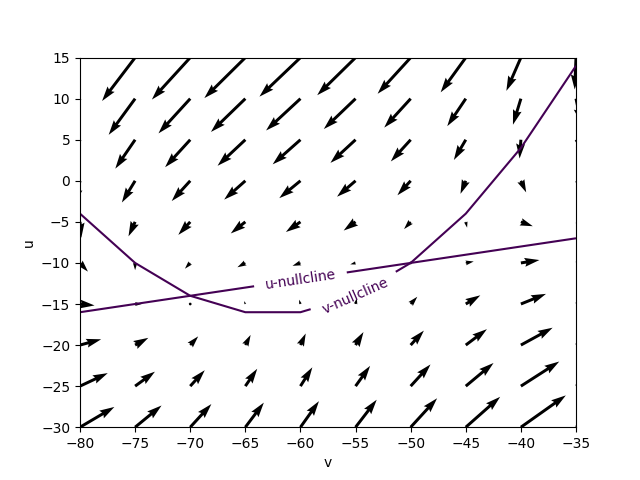
\includegraphics[scale=0.8]{imgs/izPDP.png}
\caption{ Izhikievich : Plan de phase}
\label{izPDP}
\end{figure}
\clearpage
\begin{lstlisting}[caption = {Izhikievich : Définition du modèle}]
from .core import Variable, Model
v = Variable(name='v', ddt='0.04*v**2+5*v+140-u+I', init_value=-65, 
reset_value='c', unit='mV')
u = Variable(name='u', ddt='a*(b*v-u)', init_value=-15,
reset_value='u+d')
IZHIKIEVICH = Model(v, u, spike_when='v>=30', max_spike_value=30, 
a=0.02, b=0.2, c=-65, d=8, I=0) 
\end{lstlisting}

\begin{lstlisting}[caption = {Izhikievich : Plan de phase}]
from snn.single.usual_models import IZHIKIEVICH as iz
import matplotlib.pyplot as plt
iz.phase_plan(('v', -80, -30), ('u', -30, 20), 
rescale=True) #interactive=True
plt.show()
\end{lstlisting}

\begin{lstlisting}[caption = {Izhikievich : Evolution du potentiel de membrane en fonction du temps pour plusieurs ensembles de paramètres}]
from snn.single.usual_models import izhi_model as iz
import matplotlib.pyplot as plt

A = [0.02, 0.02, 0.02, 0.1, 0.02, 0.02, 0.02, 0.1, 0.1]
B = [0.2, 0.2, 0.2, 0.2, 0.25, 0.25, 0.25, 0.26, 0.26]
C = [-65, -55, -50, -65, -65, -65, -65, -65, -65]
D = [8, 4, 2, 2, 2, 0.05, 0.05, 8, 8]
I = [15, 10, 10, 10, 15, 1, 1, -0.0488, -0.04]
V = [-65, -65, -65, -65, -65, -65, -90, -65, -65]

for a, b, c, d, i, vstart in zip(A, B, C, D, I, V):
iz['a'] = a ; iz['b'] = b ; iz['c'] = c ; iz['d'] = d
iz['I'] = i ; iz['v'] = vstart ; iz['u'] = b * vstart
iz.plot(100, 0.01, keep='v')
plt.gca().set_ylim(-80, 40)
plt.show()
\end{lstlisting}

\begin{figure}[!h]
\begin{minipage}[l]{.48\linewidth}
\centering
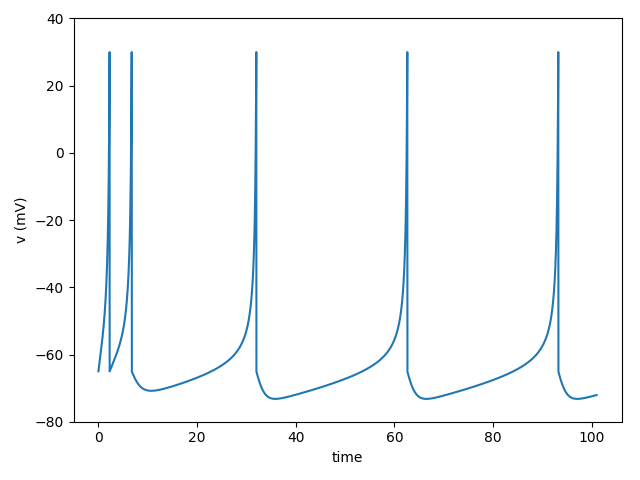
\includegraphics[scale=0.5]{imgs/izRS.png}
\caption{Izhikievich : Regular Spiking (a=0.02, b=0.2, c=-65, d=8, I=15, $v_{start}$ = -65)}
\label{izRS}
\end{minipage}\hfill
\begin{minipage}[l]{.48\linewidth}
\centering
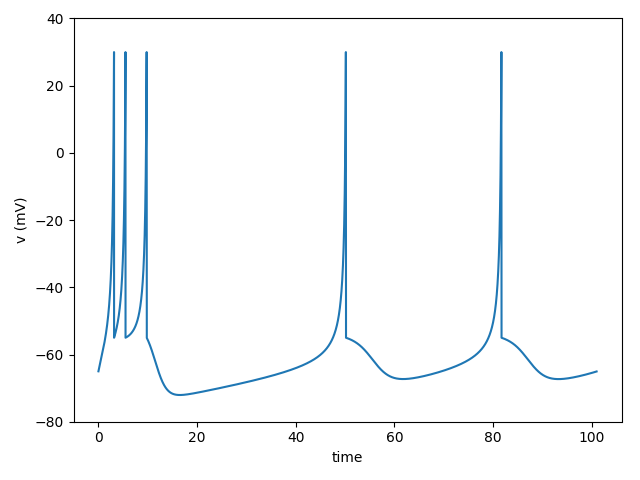
\includegraphics[scale=0.5]{imgs/izIB.png}
\caption{Izhikievich : Intrinsically Bursting (a=0.02, b=0.2, c=-55, d=4, I=10, $v_{start}$ = -65)}
\label{izIB}
\end{minipage}\hfill
\end{figure}

\begin{figure}[!h]
\begin{minipage}[l]{.48\linewidth}
\centering
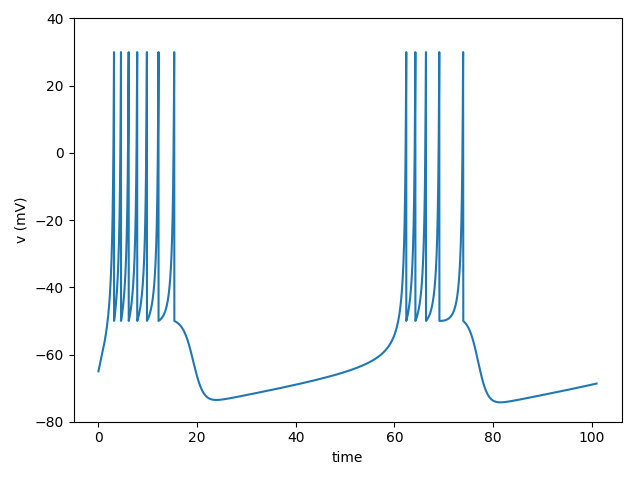
\includegraphics[scale=0.5]{imgs/izC.png}
\caption{Izhikievich : Chattering (a=0.02, b=0.2, c=-50, d=2, I=10, $v_{start}$ = -65)}
\label{izC}
\end{minipage}\hfill
\begin{minipage}[l]{.48\linewidth}
\centering
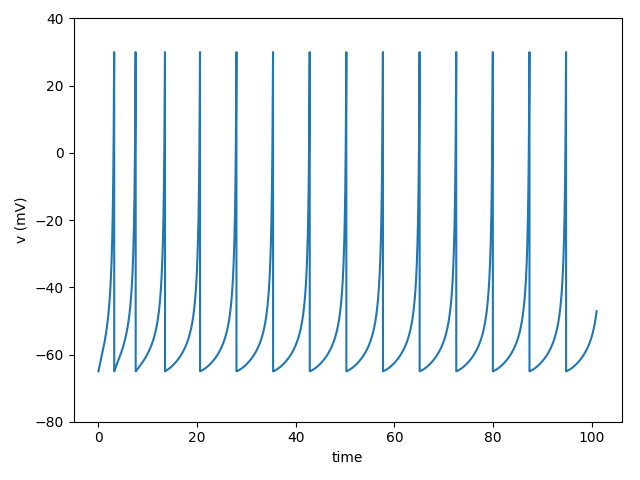
\includegraphics[scale=0.5]{imgs/izFS.png}
\caption{Izhikievich : Fast Spiking (a=0.1, b=0.2, c=-65, d=2, I=10, $v_{start}$ = -65)}
\label{izFS}
\end{minipage}\hfill
\end{figure}

\begin{figure}[!h]
\begin{minipage}[l]{.48\linewidth}
\centering
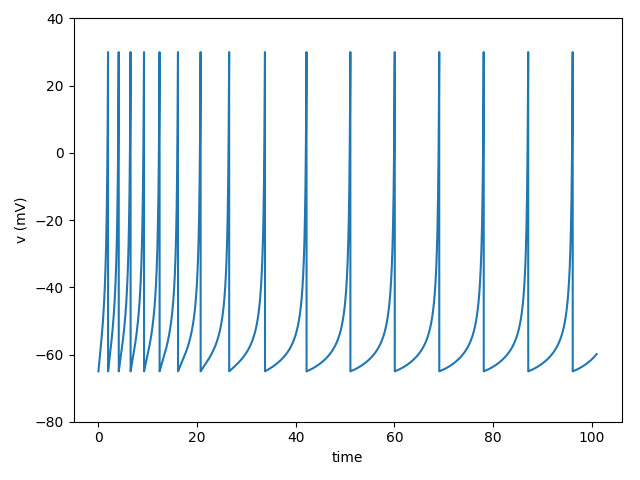
\includegraphics[scale=0.5]{imgs/izLTS.png}
\caption{Izhikievich : Low-Threshold Spiking (a=0.02, b=0.25, c=-65, d=2, I=15, $v_{start}$ = -65)}
\label{izLTS}
\end{minipage}\hfill
\begin{minipage}[l]{.48\linewidth}
\centering
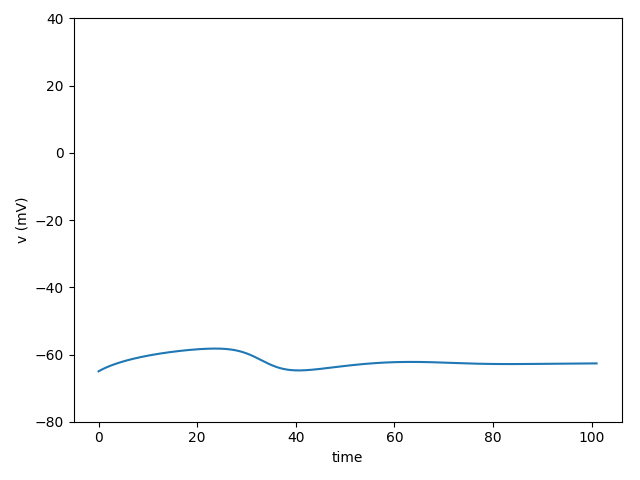
\includegraphics[scale=0.5]{imgs/izRES1.png}
\caption{Izhikievich : Resonnator (a=0.1, b=0.26, c=-65, d=8, I=-0.0488, $v_{start}$ = -65)}
\label{izRES}
\end{minipage}\hfill
\end{figure}

\begin{figure}[!h]
\begin{minipage}[l]{.48\linewidth}
\centering
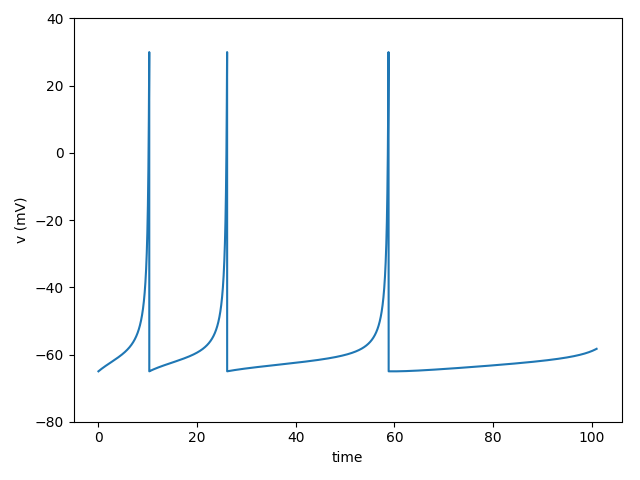
\includegraphics[scale=0.5]{imgs/izTC1.png}
\caption{Izhikievich : Thalamo-Cortical 1 (a=0.02, b=0.25, c=-65, d=0.05, I=1, $v_{start}$ = -65)}
\label{izTC1}
\end{minipage}\hfill
\begin{minipage}[l]{.48\linewidth}
\centering
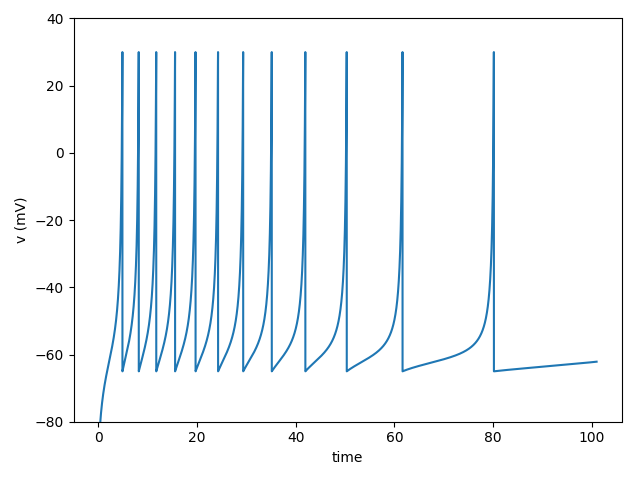
\includegraphics[scale=0.5]{imgs/izTC2.png}
\caption{Izhikievich : Thalamo-Cortical 2 (a=0.02, b=0.25, c=-65, d=0.05, I=1, $v_{start}$ = -90)}
\label{izTC2}
\end{minipage}\hfill
\end{figure}

\clearpage

\section{Modèle leaky-integrate and fire}
Ce modèle "intègre-et-tire" peut être décrit par un circuit constitué d'un ccondensateur et d'une résistance montés en parallèle. Pour déterminer l'équation caractérisant les variations du potentiel de membrane, on peut appliquer les mêmes étapes que pour le modèle de Hodgkin-Huxley en \ref{HHEQPOT}.\\

On peut donc appliquer la loi de Kirchhoff :
\setcounter{equation}{0}\begin{equation}I_C + I_R - I = 0 \label{liafeq1}\end{equation} 
avec $I$ le courant appliqué sur le neurone, $I_R$ l'intensité du courant à travers la résistance et $I_C$ l'intensité du courant au niveau du condensateur.\\

La loi d'Ohm nous donne \begin{equation}I_R = \frac{u}{R} \label{liafeq2} \end{equation} où $u$ est la tension aux bornes de la résistance.\\

Et de la définition d'un condensateur, on a 
\begin{equation} C = \frac{Q}{u} \Rightarrow I_C = C\frac{\dd u}{\dd t} \label{liafeq3}\end{equation} où C est la capacité du condensateur et Q la charge du condensateur.\\

Et en introduisant \ref{liafeq2} et \ref{liafeq3} dans \ref{liafeq1}, on a \begin{equation}C\frac{\dd u}{\dd t} = -\frac{u(t)}{R} + I(t) \nonumber \end{equation}
Que l'on peut écrire : \begin{equation}\tau_m\frac{\dd u}{\dd t} = -u(t) + RI(t) \label{LIAFEQ}\end{equation} avec $\tau_m = RC$ la constante de temps associée à la membrane.\\

Dans ce modèle, il est nécessaire d'introduire une règle pour savoir lorsque le système à produit un potentiel d'action, et une règle de réinitialisation du potentiel du membrane après un potentiel d'action.\\
On dit que le système a produit un potentiel d'action au temps $t_{PA}$ si $u(t_{PA}) \geq \eta$.\\
Et la règle de réinitialisation du potentiel de membrane après un potentiel d'action est : 
\begin{empheq}{align}\begin{split}\text{Si } u \ge \eta , \text{ al}&\text{ors : } \\ u \leftarrow u_r \end{split}\end{empheq}

Il est également courant d'introduire dans ce modèle une variation de la règle de réinitialisation du potentiel de membrane ayant pour but de modéliser la période réfractaire absolue. On introduit alors le paramètre $\Delta^{abs}$ exprimé en millisecondes, et la règle de réinitialisation devient 
\begin{empheq}{align}\begin{split}\text{Si } u \ge \eta , \text{ al}&\text{ors : } \\ &u \leftarrow u_r \\ &\frac{\dd u}{\dd t} = 0 \text{ pendant } \Delta^{abs} \text{ ms}, \\ &\text{Puis après } \Delta^{abs} \text{ ms on reprend } \frac{\dd u}{\dd t} \text{ comme définie par l'équation \ref{LIAFEQ}} \end{split}\end{empheq}

Des valeurs courantes pour les paramètres sont : $\tau_m = 10 ms, R=1, u_r=0, I=1.5, \eta=1$.\\

Ce modèle très simple est capable de simuler la base des comportements des neurones, comme on peut le voir sur la figure \ref{liaf}. Sa simplicité le rend très rapide à simuler ce qui en fait un modèle populaire dans les projets impliquant de simuler un grand nombre de neurones. Cependant, c'est un modèle purement phénoménologique, sans réelles justifications physiologiques ; et la variété des comportements que ce modèle est capable de simuler est assez faible.

\begin{lstlisting}[caption = {Leaky Integrate-and-fire : Définition du modèle}]
u = Variable(name='u', init_value=0,
ddt = '(1/tau_m)*(-u+R*I)', reset_value='ur', unit='mV')
LEAKY_INTEGRATE_AND_FIRE = Model(u, spike_when='u>=1',
max_spike_value=1, tau_m=10, R=1, ur=0, I=1.5)
\end{lstlisting}
\begin{lstlisting}[caption = {Leaky Integrate-and-fire : Evolution du potentiel de membrane en fonction du temps}]
from snn.single.usual_models import LEAKY_INTEGRATE_AND_FIRE as liaf
import matplotlib.pyplot as plt
liaf.plot(100, 1, keep='u')
plt.show()
\end{lstlisting}

\begin{figure}[!h]
\centering
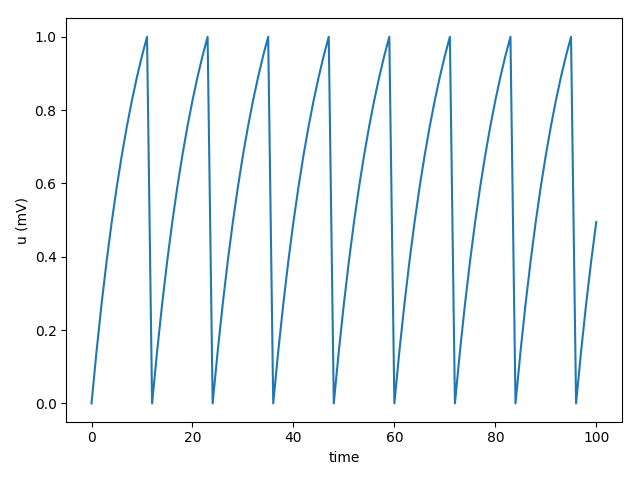
\includegraphics[scale=0.5]{imgs/liaf.png}
\caption{Leaky Integrate-and-fire : Evolution du potentiel de membrane au cours du temps pour $I = 1.5$}
\label{liaf}
\end{figure}

\pagebreak

\part{Réseau de neurones}

\section{Modèles de synapses}

\subsection{Quelques élements de neurobiologie}
Dans cette parie nous allons rappeler schématiquement la manière dont les neurones biologiques sont connectés entre eux pour former des réseaux. Une connexion entre deux neurones est appelée une synapse. Dans le système nerveux humain, il existe deux types de synapses : les synapses électriques et les synapses chimiques. Les synapses électriques permettent la transmission directe de l'influx nerveux à travers ce qu'on appelle des jonctions communicantes, tandis que les synapses chimiques ont un fonctionnement beaucoup plus complexe et permettent la modulation du potentiel de membrane du neurone post-synaptiques à partir de celui du neurone pré-synaptique par l'intermédiaire d'une communication chimique entre les deux neurones basées sur des agents que l'on appelle des neurotransmetteurs. Dans cette partie nous allons surtout nous intéresser principalement au fonctionnement des synapses chimiques : il s'agit du type de synapses dominant dans le cerveau, leur fonctionnement est complexe et elles sont supposé entre à la base des mécanismes de plasticité cérébrale et d'apprentissage.\\

On peut décomposer schématiquement les mécanismes à l'œuvre dans la transmission synaptique en 5 étapes :
\begin{enumerate}
\item Arrivée du potentiel d'action dans le bouton synaptique du neurone pré-synaptique;
\item Ouverture de canaux calciques potentiel-dépendants dans le bouton synaptique, entrée d'ions calciques dans le bouton synaptique ;
\item Migration et fusion des vésicules synaptiques contenues dans le bouton synaptique du neurone pré-synaptique et contenant les neurotransmetteurs avec la membrane, exocytose des neurotransmetteurs dans la fente synaptique;
\item Fixation de certains neurotransmetteurs sur les récepteurs associés sur les épines dendritiques du neurone post-synaptique;
\item Ouverture de canaux ioniques au niveau des dendrites du neurone post-synaptique
\begin{enumerate}
\item [5.1] Dans le cas d'une synapse excitatrice, on peut par exemple avoir l'ouverture de canaux sodiques, et l'entrée d'ions sodiques dans la cellule provoque une dépolarisation locale dans le neurone post-synaptique, que l'on appelle potentiel post-synaptique excitateur, pouvant aboutir à la création d'un potentiel d'action dans le neurone post-synaptique si la dépolarisation locale dépasse un certain seuil;
\item [5.2] Dans le cas d'une synapse inhibitrice, on peut par exemple avoir l'ouverture de canaux potassiques, et la sortie d'ions potassiques dans la cellule provoque une hyperpolarisation locale dans le neurone post-synaptique, que l'on appelle potentiel post-synaptique inhibiteur, rendant la création d'un potentiel d'action dans le neurone post-synaptique plus difficile.
\end{enumerate}
\end{enumerate}


\begin{figure}[!h]
\centering
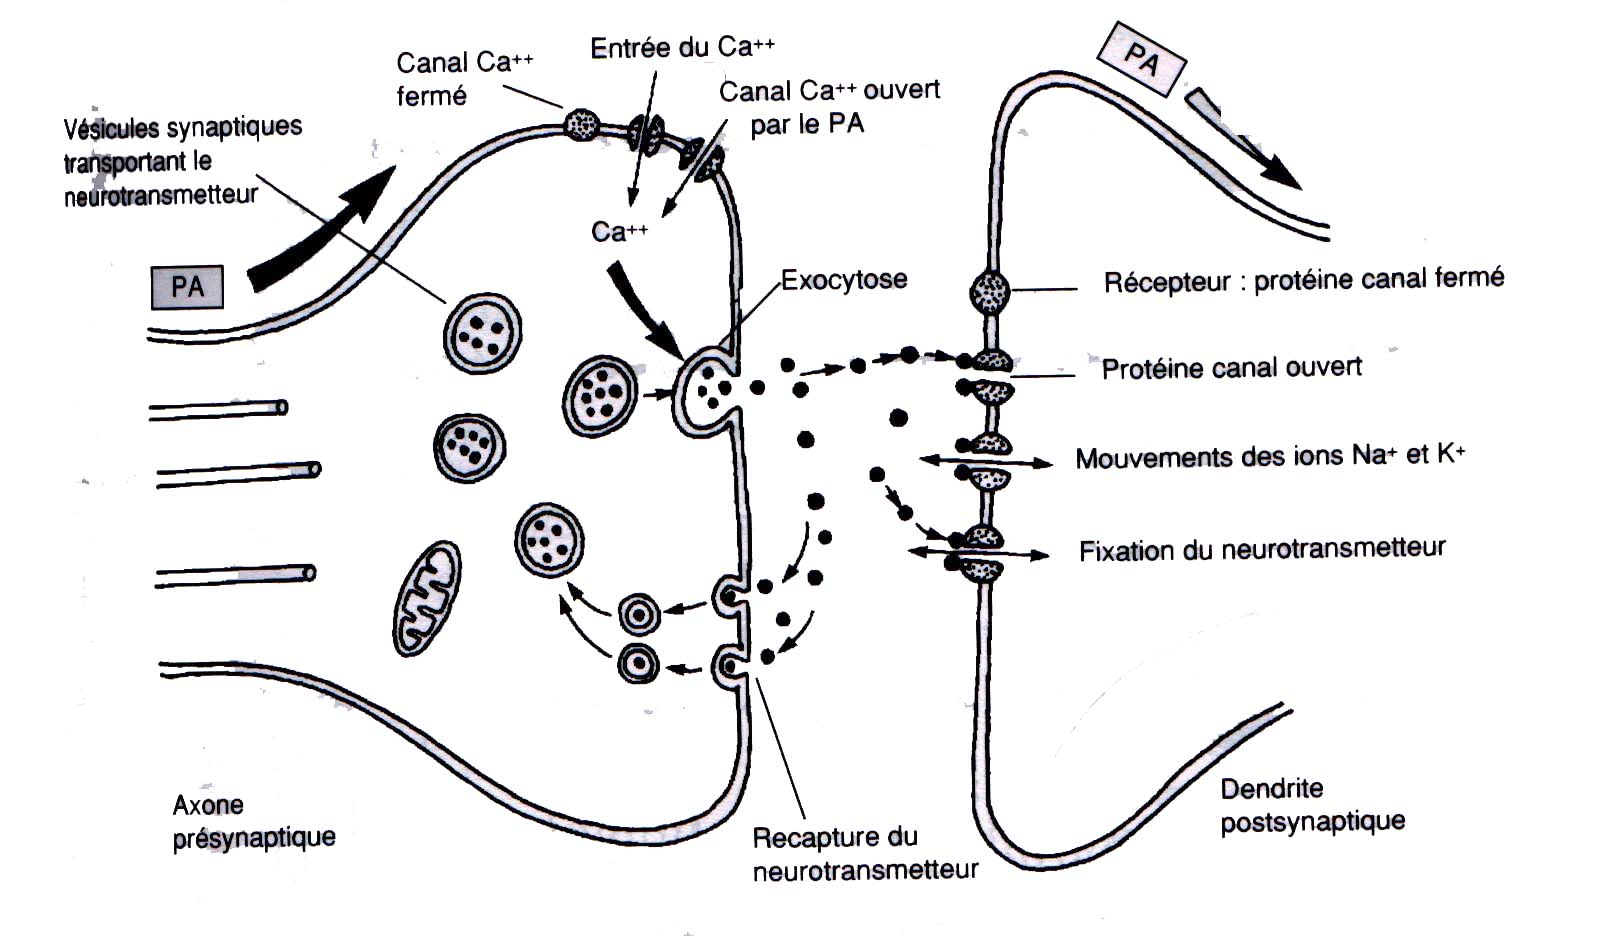
\includegraphics[scale=1.2]{imgs/3.jpg}
\caption{Une synapse \scriptsize{(https://bio.m2osw.com/gcartable/systeme\%20nerveux/synapses.htm)}}
\label{synapse}
\end{figure}


\section{Apprentissage}
\subsection{Quelques élements de neurobiologie}

\section{Justification de l'utilisation de la bibliothèque tensorflow comme base pour l'implémentation de SNN}
Tensorflow (https://www.tensorflow.org/) est une bibliothèque de computation optimisée et parallèle, écrite en C++ avec une interface de developpement python. Cette bibliothèque est particulièrement utilisée pour des applications en apprentissage machine, surtout en deep learning, et elle a souvent la réputation d'être spécifiquement dédiée ces champs d'applications, mais elle peut vraiment être utilisée pour n'importe quel projet où il est nécessaire d'avoir un grand nombre d'opérations élémentaires, et où le parallèlisme semble pertient. De plus tensorflow permet l'utilisation de plusieurs CPU ou de plusieurs GPU pour accélerer les calculs, ce qui est un élement non-négligeable, notamment, les GPU sont particulièrement efficaces pour effectuer des calculs matriciels, de par leur grande capacité de calcul parallèle.\\


Tensorflow utilise un principe appellé diagramme de flux de données (de l'anglais dataflow graph) dont le fonctionnement et les avantages sont certainemet le mieux décrits par les créateurs de tensorflow (traduction libre) : \footnote{\textit{Portions of this page are modifications based on work created and shared by Google and used according to terms described in the Creative Commons 3.0 Attribution License. See https://www.tensorflow.org/programmers\_guide/graphs for the original content} Une portion de cette page est basée sur des modifications d'un travail créé et partagé par Google et utilisé en accord avec les termes décrits dans la Creative Commons 3.0 Attribution License. Voir https://www.tensorflow.org/programmers\_guide/graphs pour le contenu originel }

\textit{Les diagrammes de flux de données sont des modèles couramment utilisés dans le calcul numérique parallèles. Dans un diagramme de flux de données, les noeuds représentent des opérations, et les flèches représentent des données utilisées ou produites par une opération. Par exemple, l'opération de multiplication correspondrait à un noeuds avec des flèches afférentes (les elements à multiplier) et une flèche efferentes (le résultat de la multiplication).
Les diagrammes de flux de données ont plusieurs avantages que tensorflow utilises lors de l'execution d'un programme :
\begin{itemize}
\item \textbf{Le parallèlisme.} En utilisant les flèches pour réprésenter la dépendance entre les opérations, il est facile pour le système d'identifier les opérations qui peuvent être effectuées en parallèle
\item\textbf{L'execution distribuée.} En utilisant les flèches pour représenter les valeur qui circulent entre les opérations, il est possible pour tensorflow de partitionner le programme entre plusieurs hardware (CPUs, GPUs et TPUs) sur différentes machines. Tensorflow gère la communication et la coordination necessaire entre les composants.
\item\textbf{Compilation.}  Tensorflow utilise un compilateur XLA (Accelerated Linear Algebra) qui peut utiliser les informations dans le diagramme de flux de données pour générer un code plus rapide, par exemple, en fusionnant les opérations adjacentes dans le diagramme.
\item\textbf{Portabilté. } Un diagramme de flux de données est une représentation du code du modèle indépendante du language de programmation. Ainsi, on peut construire un diagramme de flux de données en Pyton, le sauvegarder, puis le restaurer dans un code en C++ pour améliorer les performances
\end{itemize}}

\begin{figure}[!h]
\centering
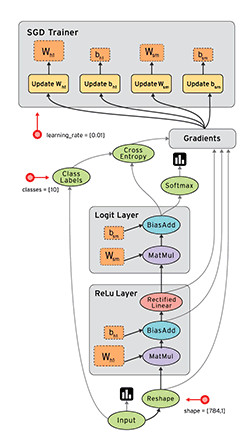
\includegraphics[scale=0.6]{imgs/4.jpg}
\caption{Représentation graphique d'un diagramme de flux de données \scriptsize{(https://www.tensorflow.org/programmers\_guide/graphs)}}
\label{synapse}
\end{figure}

Pour justifier l'utilisation de tensorflow, il peut être utile de comparé ses performances à celles d'une des bibliothèques de calcul scientifique les plus populaires pour python : numpy.\\
Afin d'estimer cette différence de performances entre ces deux bibliothèques dans la tâche de simuler des réseaux de spiking-neurons, j'ai créé deux implémentation du même réseau simple, une basée sur numpy, l'autre sur tensorflow. \\

Les caractéristiques du réseau sont les suivantes :
\begin{itemize}
\item On utilise le modèle de Izhiekievich pour modéliser les neurones, avec une création des paramètres du modèle orientée dans l'idée d'avoir une grande diversité de comportements neuronaux;
\item L'architecture du réseau est de type entiremment interconnectée, c'est-à-dire que chaque neurone est connecté avec tout les autres;
\item Les synapses sont des synapses à poids simples sans délai, c'est-à-dire que l'entrée interne de chaque neurone est égal à la somme des poids afférents des neurones ayant déchargés à l'étape précédente.
\end{itemize}

Les deux implémentations sont voulues équivalentes en termes de comportements et utilisant au mieux l'arsenal fournit par les deux bibliothèques. Notamment, sur la manière de calculer la communication interne entre les neurones du réseau, 
la méthode de traitement optimale diffère entre numpy et tensorflow. Dans les deux cas, on souhaite récupérer le vecteur $I_{interne} = (I_j)_{1\leq j \leq n}$ qui définie la part propre au réseau de l'input de chaque neurones.\\
On a alors deux manières de calculer $I_{interne}$:\\
Soit $W=(w_{ij})_{ij}$ la matrice donnant les poids des connexions, avec $w_{ij}$ le poids de la connexion entre le neurone $i$ et le neurone $j$.
\begin{enumerate}
\item Soit $F$ l'ensemble des indices des neurons qui ont produit un potentiel d'action à l'étape $n-1$, alors \begin{center} $I_j = \displaystyle \sum_{i\in F} w_{ij}$ \end{center}
Ou, dit autrement, on somme les lignes de W correspondant aux neurones qui ont déchargé, colonnes par colonnes.
\item Soit $f=(f_i)_i$ le vecteur défini par $f_i = \left\{\begin{array}{l} 1 \text{ si le neurone i à déchargé } \\ 0 \text{ sinon } \end{array}\right.$, alors \begin{center} $I_{interne} = \displaystyle W^T\dot f$ \end{center}
\end{enumerate}

L'approche 1., basé sur l'indiçage, s'est révélé la plus efficace pour numpy, tandis que l'approche 2., basé sur la multiplication de matrice, s'est révélée plus efficace pour tensorflow.\\

Les codes des deux implémentations sont présentés ci-dessous. La version basée sur tensorflow n'utilise pas l'outil construit dans ce travail, pour rester complètement transparent sur l'équivalence des deux codes. \\Ces codes ont été exécutés sur le \textit{hardware} suivant :
\begin{itemize}
\item Processeur (CPU) : Intel(R) Core(TM) i7-4700HQ CPU \@ 2.40GHz 2.40GHz
\item Carte graphique (GPU) : NVIDIA GeForce GTX 850M
\end{itemize}
Le \textit{hardware} sur lequel est executé ces codes est déterminant dans les résultats sur la différence des temps de computation : en effet, numpy n'utilise que le CPU pour faire ses calculs tandis que tensorflow utilise également la GPU.

\clearpage
\begin{lstlisting}[caption = {Numpy vs Tensorflow : Implémentation Numpy}]
import numpy as np


def build(n, exi_inhi_rate, Iext, seed=123):
    """Build parameters, weight matrix and variable init states"""

    np.random.seed(seed)

    nb_ex = round(n * exi_inhi_rate)
    nb_in = round(n * (1 - exi_inhi_rate))

    # Parameters generation as in (Izhikievich, 2003) in order to have
    # a variety of neural behavior
    re = np.array(np.random.rand(nb_ex, 1), dtype=np.float32)
    ri = np.array(np.random.rand(nb_in, 1), dtype=np.float32)
    a = np.array(np.concatenate((0.02 * np.ones((nb_ex, 1)),
                                 0.02 + 0.08 * ri)), dtype=np.float32)
    b = np.array(np.concatenate((0.2 * np.ones((nb_ex, 1)),
                                 0.25 - 0.05 * ri)), dtype=np.float32)
    c = np.array(np.concatenate((- 65 + 15 * re ** 2,
                                 - 65 * np.ones((nb_in, 1)))),
                 dtype=np.float32)
    d = np.array(np.concatenate((8 - 6 * re ** 2,
                                 2 * np.ones((nb_in, 1)))),
                 dtype=np.float32)

    # Weight matrix generation W =(wij) wich give the weight 
    # of the connexion between the neuron i and the neuron j
    # Excitator neurons have positive weights between 0 and 0.5
    # Inhibitor neurons have negative weights between -1 and 0
    W = np.random.rand(n, n)
    W[:nb_ex, :] *= 0.5
    W[nb_ex:, :] *= -1
    W = np.array(W, dtype=np.float32)

    # Initialisation state of the variables
    v = - 65 * np.ones((n, 1), dtype=np.float32)
    u = np.multiply(b, v)
    fired = np.zeros(n, dtype=np.bool)
    I = Iext(0)

    return a, b, c, d, W, v, u, I, fired


def simulate(T, dt, a, b, c, d, W, v, u, I, fired, Iext, seed=123):
    """Simulate the numpy model for T seconds with dt time step using 
       parmeters from build and where Iext is the function of time 
       which give the external current injected for each time 0<=t<T"""

    np.random.seed(seed)

    M = int(T / dt)

    # Initialization of the matrixes containg the states
    vs, us, Is, fireds = v.T, u.T, I.T, {0: fired}

    for m in range(M - 1):

        # Reset rule
        u[fired] = u[fired] + d[fired]
        v[fired] = c[fired]

        # The dynamical system
        u = u + dt * (a * (b * v - u))
        v = v + dt * (((0.04 * v) + 5) * v + 140 - u + I)

        # Get indexes of neurons that fired
        fired = np.where(v >= 30)[0]

        # Keep all neurons that fired at 30mV
        v[fired] = 30

        # Update the input, according to external input and to
        # internal influence of neurons that fired, 
        # wich is computed by summing by columns all raw of W
        # with indexes corresponding to those of neurons that fired
        I = Iext(m * dt)+np.sum(W[fired, :], axis=0, keepdims=True).T

        # Storing states
        Is = np.vstack((Is, I.T))
        vs = np.vstack((vs, v.T))
        us = np.vstack((us, u.T))
        fireds[m * dt] = fired.copy()

    return (np.array(vs, dtype=np.float32),
            np.array(us, dtype=np.float32),
            np.array(Is, dtype=np.float32), fireds)

\end{lstlisting}

\begin{lstlisting}[caption = {Numpy vs Tensorflow : Implémentation Tensorflow}]
import tensorflow as tf
import numpy as np


def build(n, exi_inhi_rate, dt, Iext, seed=123):
    """Crating tf graph for simple network used in test np vs tf"""

    np.random.seed(seed)

    n_exi = round(n * exi_inhi_rate)
    n_inhi = round(n * (1 - exi_inhi_rate))

    graph = tf.Graph()
    with graph.as_default():

        # Parameters generation as in (Izhikievich, 2003) in order to 
        # have a variety of neural behavior
        re = tf.Variable(np.random.rand(n_exi, 1), dtype=tf.float32)
        ri = tf.Variable(np.random.rand(n_inhi, 1), dtype=tf.float32)
        a = tf.Variable(tf.concat([0.02 * tf.ones((n_exi, 1)),
                                0.02 + 0.08 * ri], 0),dtype=tf.float32)
        b = tf.Variable(tf.concat([0.2 * tf.ones((n_exi, 1)),
                                0.25 - 0.05 * ri], 0),dtype=tf.float32)
        c = tf.Variable(tf.concat([-65 + 15 * re ** 2,
                                -65 * tf.ones((n_inhi, 1))], 0),
                        dtype=tf.float32)
        d = tf.Variable(tf.concat([8 - 6 * re ** 2,
                                2 * tf.ones((n_inhi, 1))], 0),
                        dtype=tf.float32)

        # Weight matrix generation W =(wij) wich give the weight of the 
        # connexion between the neuron j and the neuron i
        # Excitator neurons have positive weights between 0 and 0.5
        # Inhibitor neurons have negative weights between -1 and 0
        W = np.random.rand(n, n)
        W[:n_exi, :] *= 0.5
        W[n_exi:, :] *= -1
        W = tf.Variable(W.T, dtype=tf.float32)

        # Initialisation state of the variables
        v = tf.Variable(-65 * tf.ones((n, 1)), dtype=tf.float32)
        u = tf.Variable(tf.multiply(b, v), dtype=tf.float32)
        fired = tf.Variable(tf.zeros((n, 1), dtype=tf.bool))
        I = tf.Variable(Iext(0), dtype=tf.float32)

        # Reset rule
        new_v = tf.where(fired, c, v)
        new_u = tf.where(fired, tf.add(u, d), u)

        # The dynamical system
        dv = tf.add(tf.subtract(tf.add(tf.multiply(tf.add(
                tf.multiply(0.04, new_v), 5.0), new_v), 140),new_u),I)
        new_v = np.add(new_v, np.multiply(dv, dt))
        du = tf.multiply(a, tf.subtract(tf.multiply(b, new_v), new_u))
        new_u = np.add(new_u, np.multiply(du, dt))

        # Get a boolean vector of neurons that fired
        v30 = tf.Variable(30 * tf.ones((n, 1)), dtype=tf.float32)
        fired_op = fired.assign(tf.greater_equal(new_v, v30))

        # Keep all neurons that fired at 30mV
        v_reseted = tf.where(fired_op, v30, new_v)
        v_op = v.assign(v_reseted)
        u_op = u.assign(new_u)

        # Update the input, according to external input and to
        # internal influence of neurons that fired, 
        # wich is computed by doing W.f with f=(fi) the n-tuple
        # with fi = 1 if neuron i fired else fi = 0
        external_input = tf.placeholder(tf.float32, shape=(n, 1))
        I_op = I.assign(tf.add(external_input,
                               tf.matmul(W, tf.cast(fired, tf.float32))))

        return graph,v,u,I,v_op,u_op,fired_op,I_op,external_input


def simulate(T, dt, graph, v, u, I, external_input, Iext,
             v_op, u_op, fired_op, I_op, seed=123):
    """Simulate the tf model for T seconds with dt time step 
       using parmeters from build and where Iext is the function
       of time which give the external current injected for each 
       time 0<=t<T"""

    np.random.seed(seed)

    with tf.Session(graph=graph) as sess:
        M = int(T / dt)
        sess.run(tf.global_variables_initializer())

        # Getting initialization values
        v, u, I = sess.run([v, u, I])

        # Initialization of the matrixes containg the states
        vs, us, fireds, Is = [v, ], [u, ], {0: np.array([])}, [I, ]

        for m in range(M - 1):

            # Running the simulation, inputing the external current
            # and getting current stat for the variables and neurons
            # that fired
            v, u, fire, I = sess.run([v_op, u_op, fired_op, I_op],
                            feed_dict={external_input: Iext(m * dt)})

            # Storing states
            Is.append(I)
            vs.append(v)
            us.append(u)
            fireds[m * dt] = np.where(fire)[0]

    return (np.array(vs, dtype=np.float32), 
            np.array(us, dtype=np.float32),
            np.array(Is, dtype=np.float32), fireds)
\end{lstlisting}

\clearpage
Nous avons ensuite comparé les comportements de ces deux implémentations avec les paramètres (T=200, dt=0.2, exi\_inhi\_rate=0.6, n=100, Iext=$t\mapsto 5$), afin de vérifier que les deux implémentations étaient bien équivalentes, ce qui, aux méthodes d'arrondis propres aux bibliothèques prêt, c'est révélé être le cas, comme nous pouvons le voir sur les figures \ref{neuronplotnp}, \ref{neuronplottf}, \ref{rasternp} et \ref{rastertf}.\\

\begin{figure}[!h]
\begin{minipage}[l]{.48\linewidth}
\centering
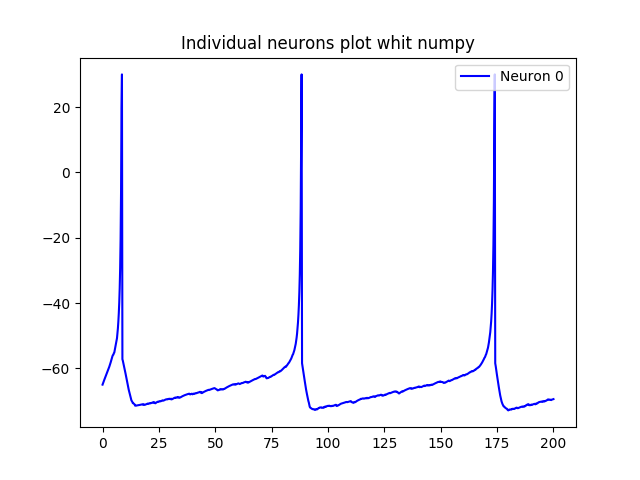
\includegraphics[scale=0.5]{imgs/neuronplotnp.png}
\caption{Numpy vs Tensorflow : Single Neuron Plot for numpy}
\label{neuronplotnp}
\end{minipage}\hfill
\begin{minipage}[l]{.48\linewidth}
\centering
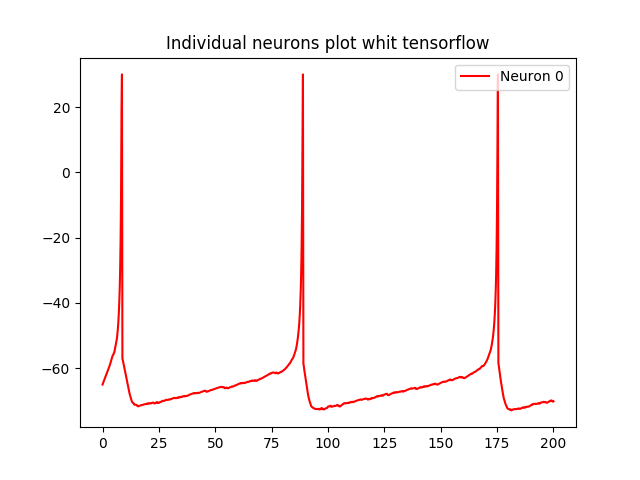
\includegraphics[scale=0.5]{imgs/neuronplottf.png}
\caption{Numpy vs Tensorflow : Single Neuron Plot for tensorflow}
\label{neuronplottf}
\end{minipage}\hfill
\end{figure}

\begin{figure}[!h]
\begin{minipage}[l]{.48\linewidth}
\centering
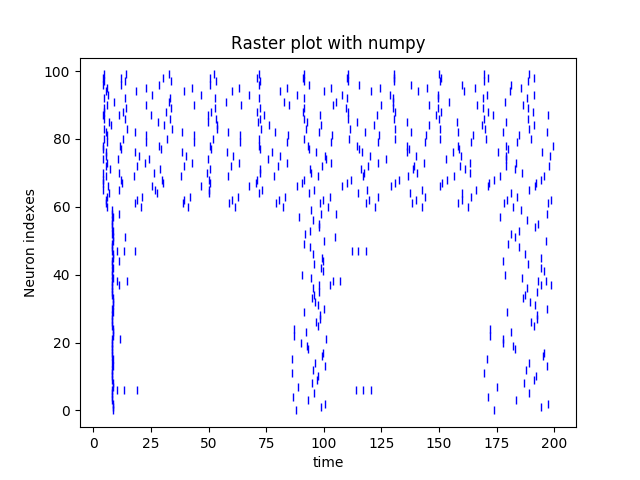
\includegraphics[scale=0.5]{imgs/rasternp.png}
\caption{Numpy vs Tensorflow : Raster Plot for numpy}
\label{rasternp}
\end{minipage}\hfill
\begin{minipage}[l]{.48\linewidth}
\centering
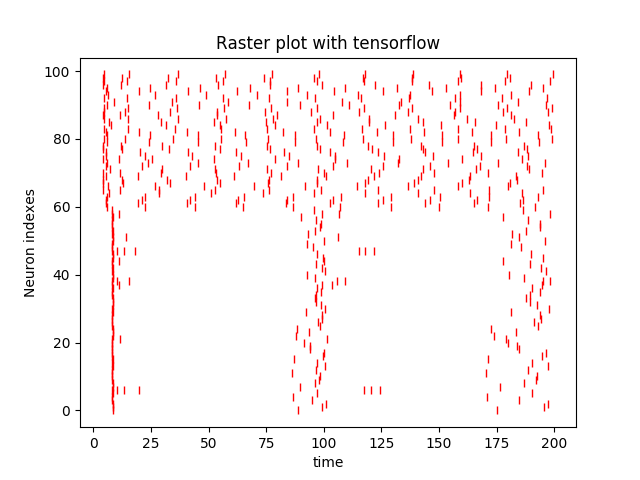
\includegraphics[scale=0.5]{imgs/rastertf.png}
\caption{Numpy vs Tensorflow : Raster Plot for tensorflow}
\label{rastertf}
\end{minipage}\hfill
\end{figure}


Enfin nous avons comparé le temps de computation de ces deux implémentations en faisant varier la taille du réseau (c'est-à-dire le nombre de synapses). Les résultats semblent montrer que pour un petit ($< \raisebox{-0ex}{\textasciitilde}10^4$) nombre de synapses, numpy est plus efficace que tensorflow, tandis que pour un grand ($>\raisebox{-0ex}{\textasciitilde}10^6$) nombre de synapses, tensorflow est plus efficace que numpy, jusqu'à être environ dix fois plus efficace pour un réseau de $\raisebox{-0ex}{\textasciitilde}10^7$ synapses.

\begin{figure}[!h]
\centering
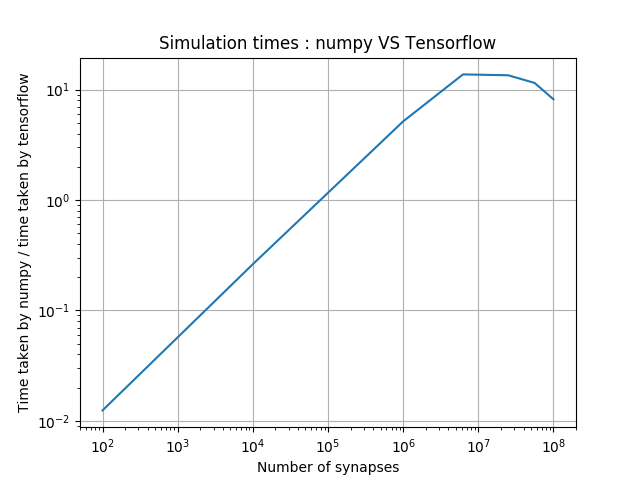
\includegraphics[scale=1]{imgs/timelogratio.png}
\caption{Numpy vs Tensorflow : Ratio  $\frac{\text{Temps de computation pour numpy}}{\text{Temps de computation pour tensorflow}}$  en fonction du nombre de synapses du réseau}
\label{timelogratio}
\end{figure}

\part{Etude de (Héricé et al., 2016) }

\part{Code}
\url{https://github.com/ArnoGranier/SNN}

\nocite{*}

\bibliographystyle{apacite}
\bibliography{ref}



\end{document}